\documentclass[a4paper,10pt,fleqn]{jarticle}
\usepackage{graphicx}
\usepackage{amssymb}
\usepackage{amsmath}
\usepackage{ascmac}
\usepackage{setspace}
\usepackage{float}
\usepackage{slashbox}
\usepackage[dvips,usenames]{color}
\usepackage{colortbl}
\usepackage{eclbkbox}
\usepackage{indent}
\usepackage{url}
\definecolor{bl}{gray}{0.8}
\definecolor{myred}{rgb}{1,0,0} 
\definecolor{mygreen}{rgb}{0,1,0} 
\definecolor{myblue}{rgb}{0,0,1} 
\definecolor{mycyan}{rgb}{0,1,1} 
\definecolor{mymagenta}{rgb}{1,0,1} 
\definecolor{myyellow}{rgb}{1,1,0} 
%--余白の設定
\setlength{\topmargin}{20mm}
\addtolength{\topmargin}{-1in}
\setlength{\oddsidemargin}{20mm}
\addtolength{\oddsidemargin}{-1in}
\setlength{\evensidemargin}{15mm}
\addtolength{\evensidemargin}{-1in}
\setlength{\textwidth}{170mm}
\setlength{\textheight}{254mm}
\setlength{\headsep}{0mm}
\setlength{\headheight}{0mm}
\setlength{\topskip}{0mm}
\makeatletter
\def\@oddhead{}
\def\@evenhead{}
\def\@evenfoot{\normalfont\rmfamily\hfil---\,\thepage\,---\hfil}
\def\@oddfoot{\normalfont\rmfamily\hfil---\,\thepage\,---\hfil}
\def\ps@titlepage{\let\@oddhead\@empty}
\def\ps@titlepage{\let\@evenhead\@empty}
\makeatother
\begin{document}
\thispagestyle{empty}
\begin{center}
\vspace{3em}
{\bf \Huge{about:R}}
\vspace{1em}\\
\today
\end{center}
\begin{indentation}{2.5cm}{2.5cm}
\begin{screen}
\tableofcontents
\end{screen}
\end{indentation}
\begin{center}
@y-system
\end{center}
\newpage
\pagenumbering{arabic}
\section{Rとは}
1996年に登場した,オープンソースでフリーの統計解析向け言語及び開発実行環境であり,最新バージョン 3.2.3 (Wooden Christmas-Tree) (2015/12/10 release).
Linux,Windows,OSX で利用可能である.
似た言語では S言語があり,Rが開発される前にAT\&Tベル研究所によって開発された統計処理言語である.

Rではさまざまな構造のデータを保持でき,記法がC言語に似ている為,習得が大変容易である.
コントリビュータによって用意されるパッケージも豊富で,その数は5000個以上である.

\section{Rをインストールしよう}
まず,{\tt http://www.r-project.org/} にアクセスし,左サイドバーの CRAN をクリックすると,CRAN のミラーサーバを選択する画面が表示されるので,なるべく日本のミラーサーバを選択する.
日本でのミラーサーバは山形大学・統計数理研究所に存在している.
オススメは統計数理研究所(Institute of Statistical Mathematics, Tokyo).

ミラーサーバにアクセスし,OSを選択する.
以下の作業は,リリースされている最新バージョンによって表示が多少異なる.
また,インストール時の画像は R3.0.2 のものである.

\subsection{Windowsの場合}
\underline{Download R for Windows} → \underline{base} → \underline{Download R 3.2.0 for Windows} (62 megabytes, 32/64 bit) の順にクリックし,インストーラをダウンロードする.

\includegraphics[width=2cm]{img/windows/win001.eps} ダウンロードしたインストーラを起動し,以下のダイアログを進めていく.


\includegraphics[width=6cm]{img/windows/win002.eps}\hspace{0.8em} 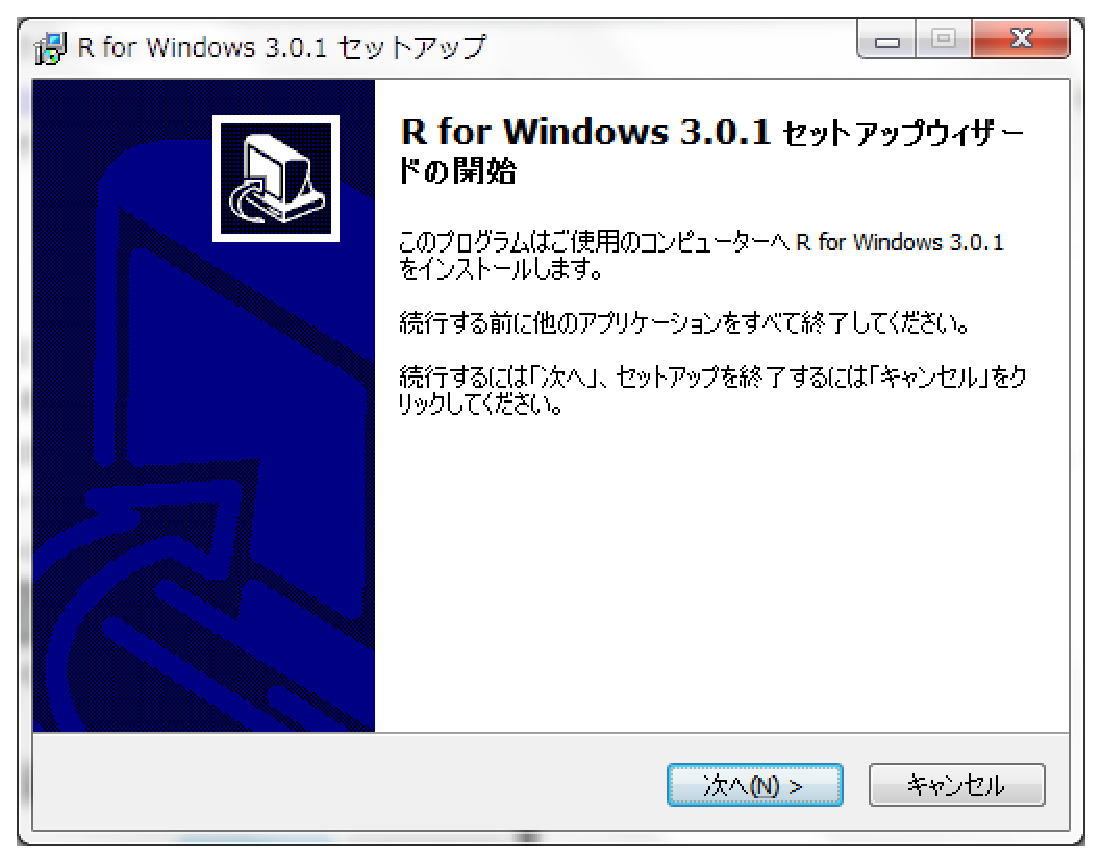
\includegraphics[width=8cm]{img/windows/win003.eps}\\

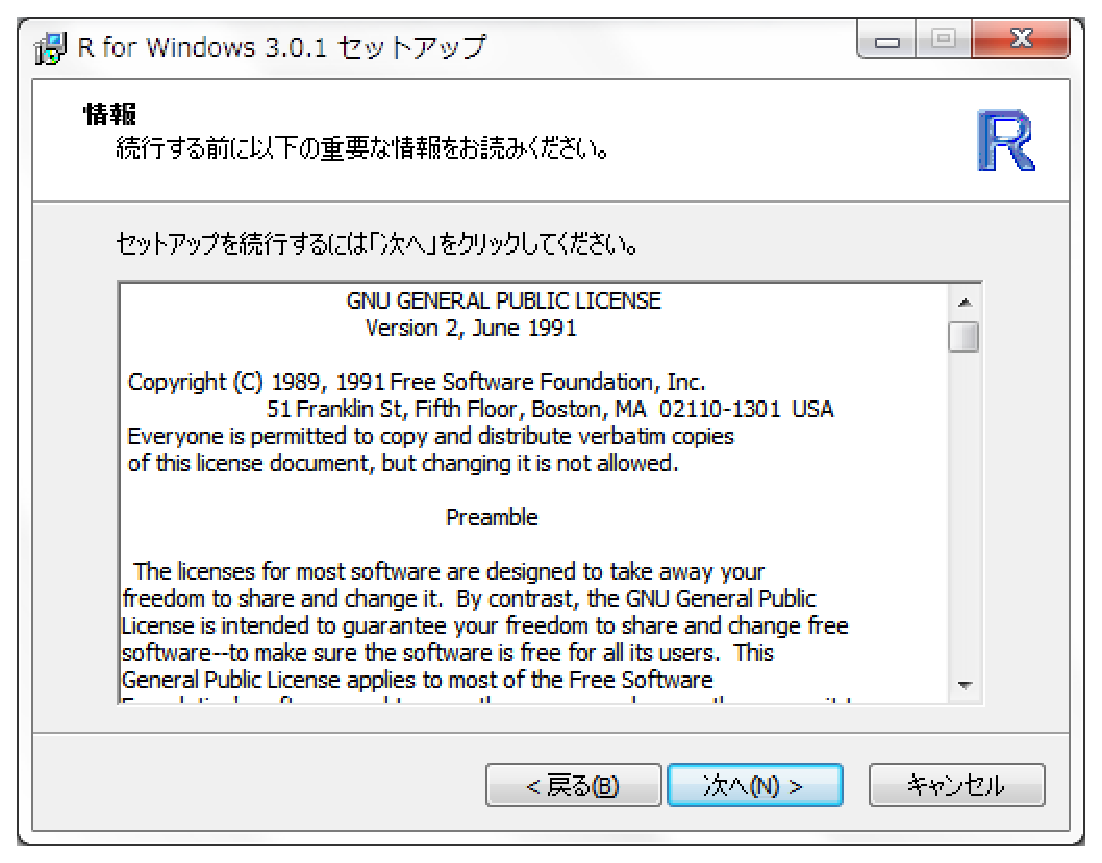
\includegraphics[width=8cm]{img/windows/win004.eps}\hspace{0.8em} 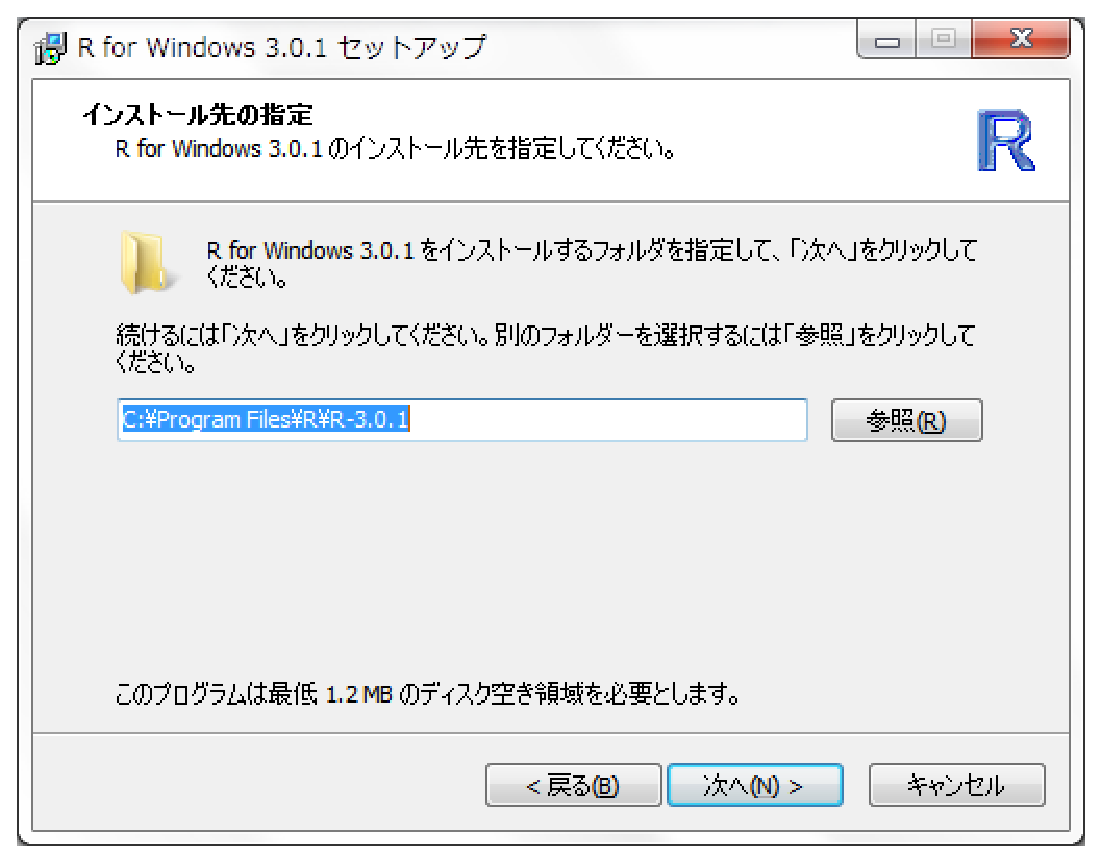
\includegraphics[width=8cm]{img/windows/win005.eps}\\

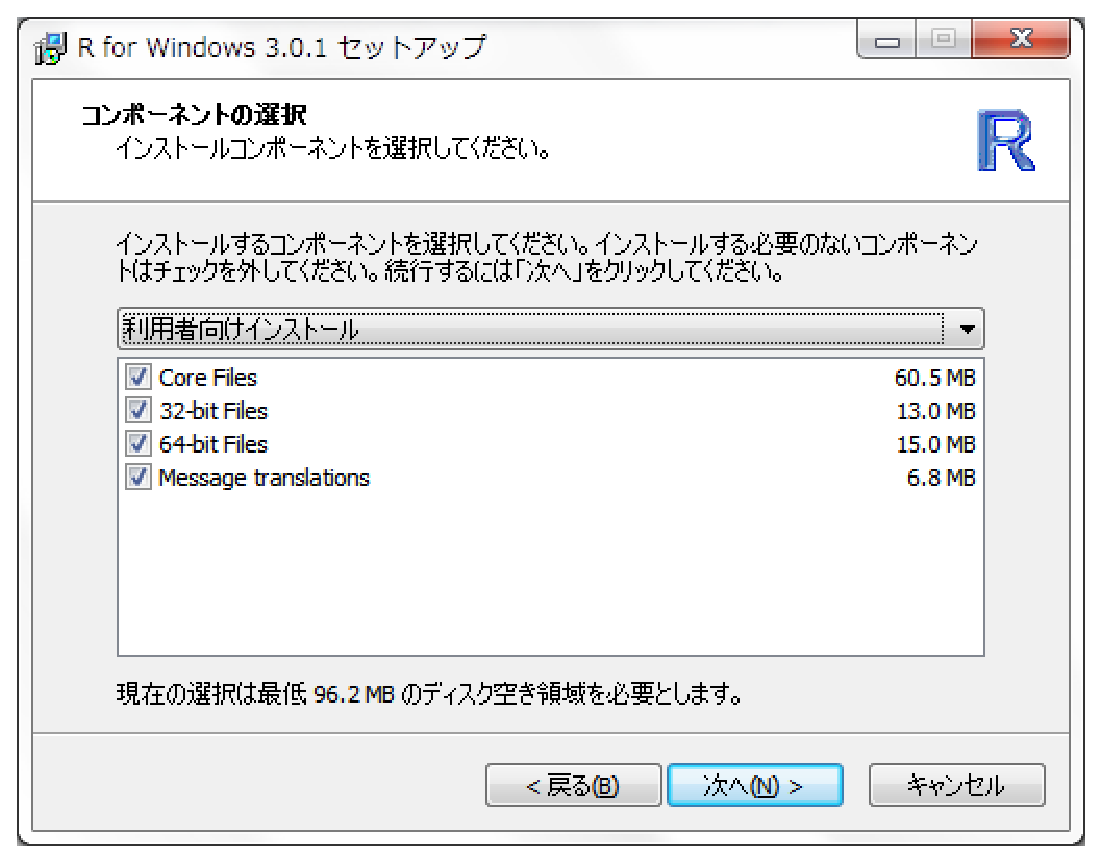
\includegraphics[width=8cm]{img/windows/win006.eps}\hspace{0.8em} 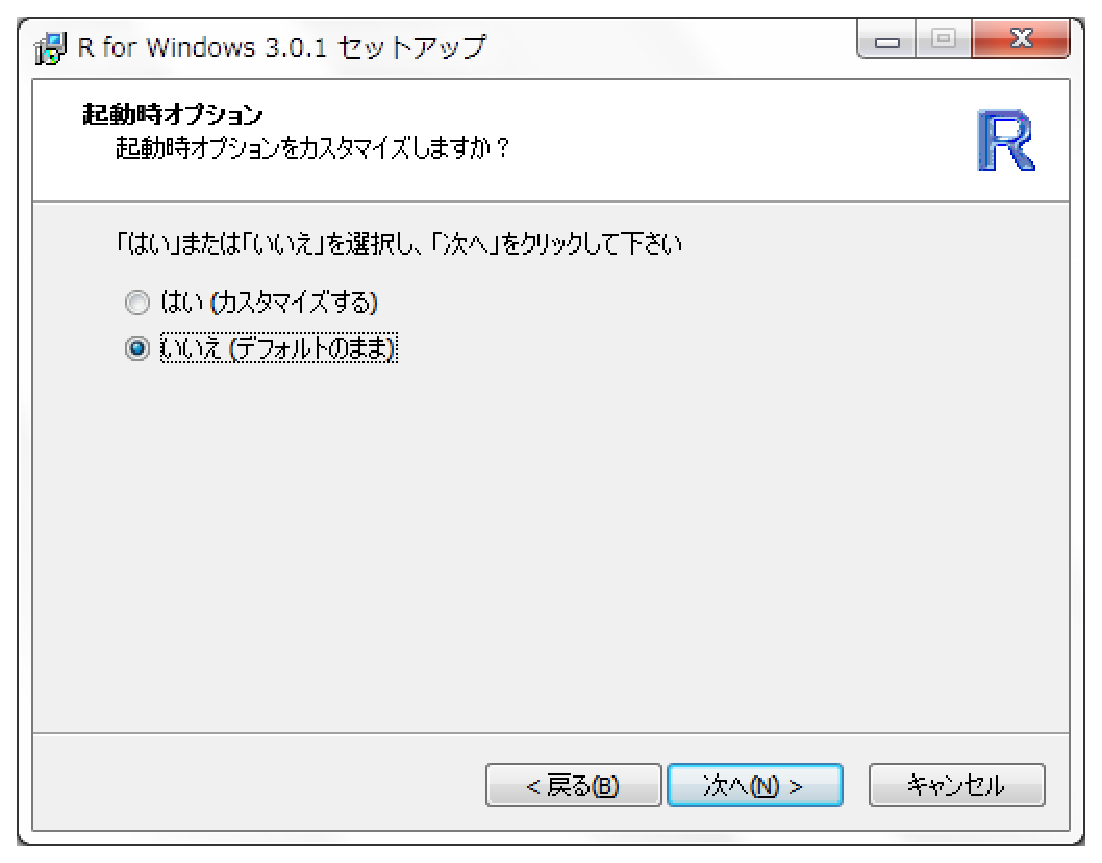
\includegraphics[width=8cm]{img/windows/win007.eps}\\

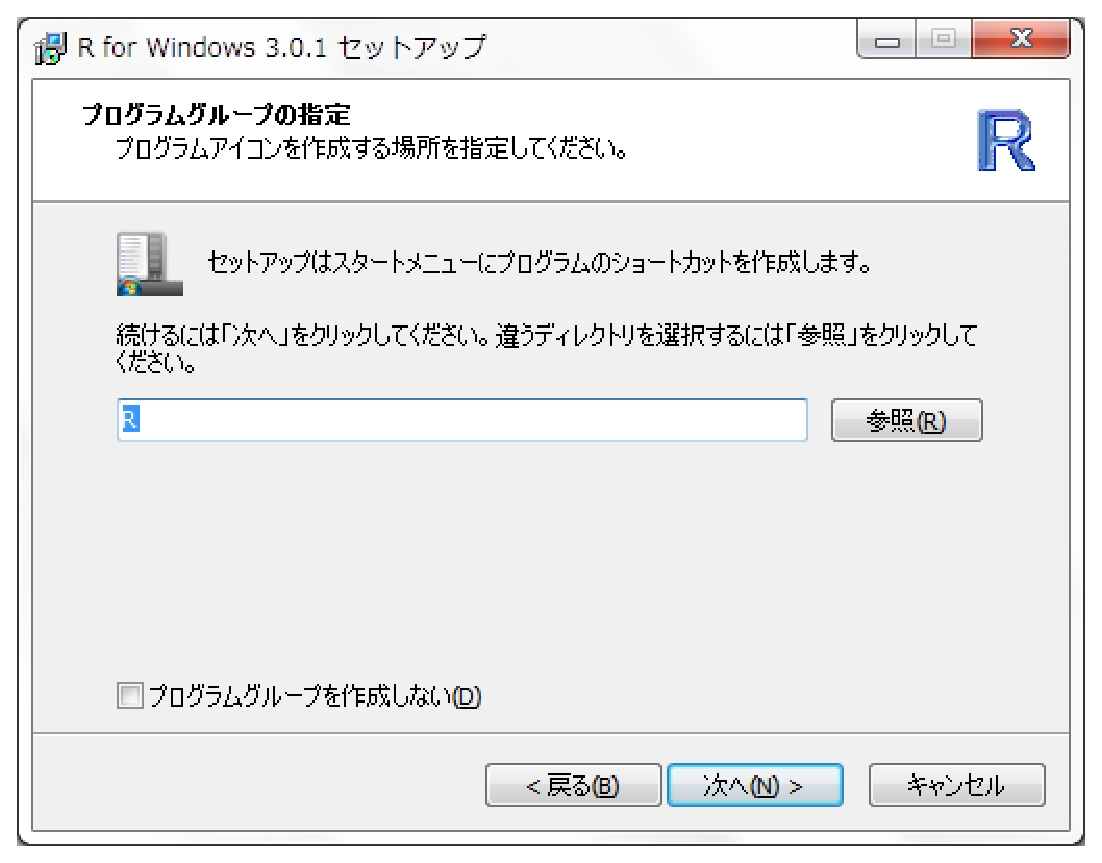
\includegraphics[width=8cm]{img/windows/win008.eps}\hspace{0.8em} 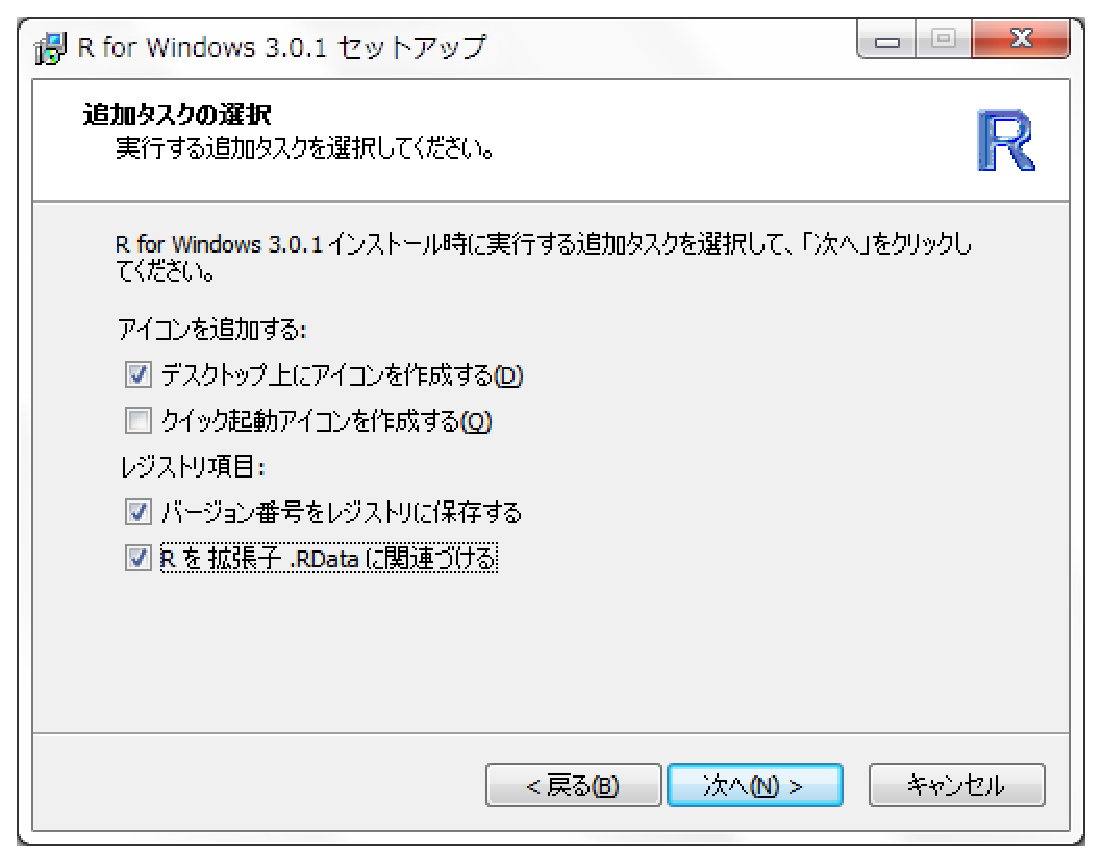
\includegraphics[width=8cm]{img/windows/win009.eps}\\

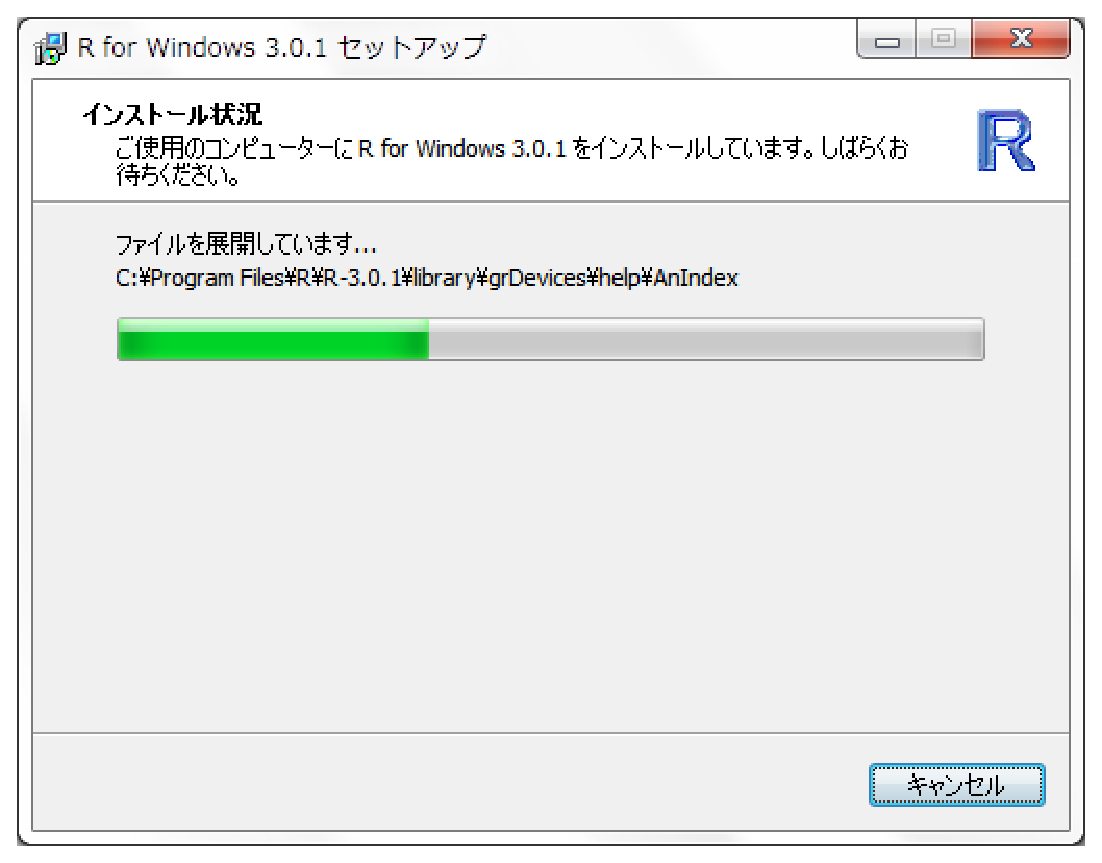
\includegraphics[width=8cm]{img/windows/win010.eps}\hspace{0.8em} 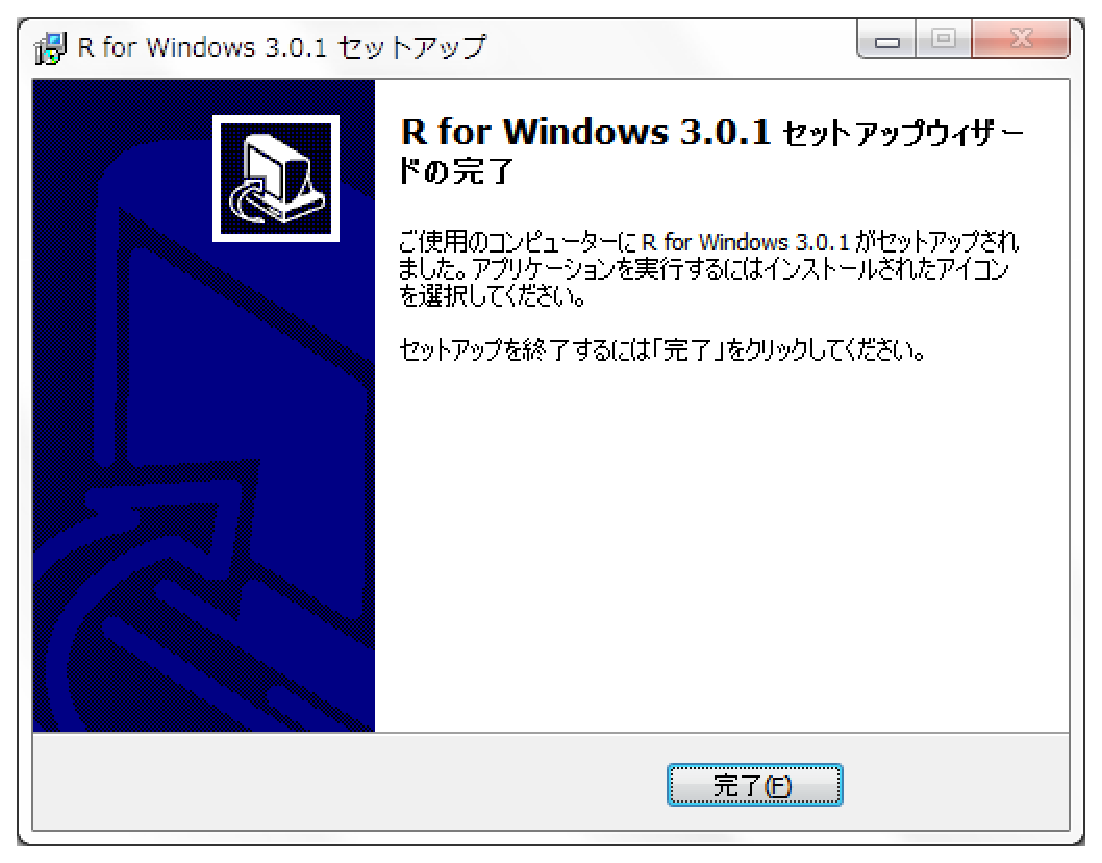
\includegraphics[width=8cm]{img/windows/win011.eps}\\

以上でインストールは完了する.\\

デスクトップに作成されたショートカット 
\includegraphics[width=1.7cm]{img/windows/win012.eps}より起動する.
\subsection{OSX (Mac)の場合}
\underline{Download R for (Mac) OS X} → \underline{R-3.2.0.pkg} の順にクリックし,インストーラをダウンロードする.\\
OS が古い場合は\underline{R-3.1.3-snowleopard.pkg}を用いてインストールする.

\includegraphics[width=1.8cm]{img/osx/osx001.eps} ダウンロードしたインストーラを起動し,以下のダイアログを進めていく.\\

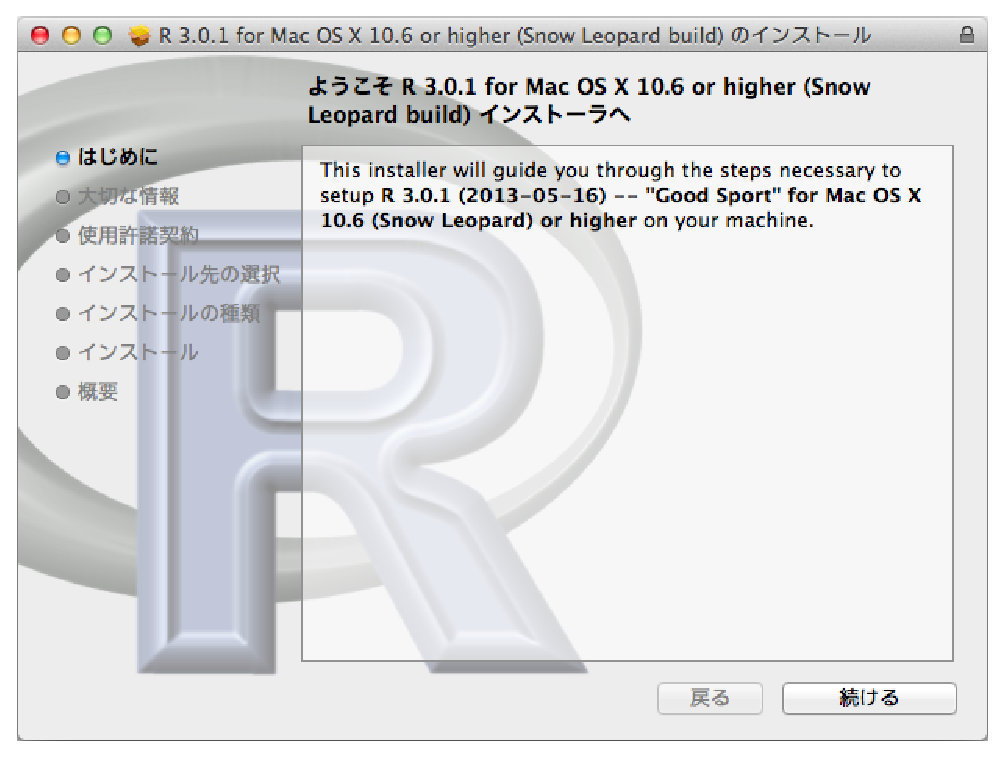
\includegraphics[width=8cm]{img/osx/osx002.eps}\hspace{0.8em} 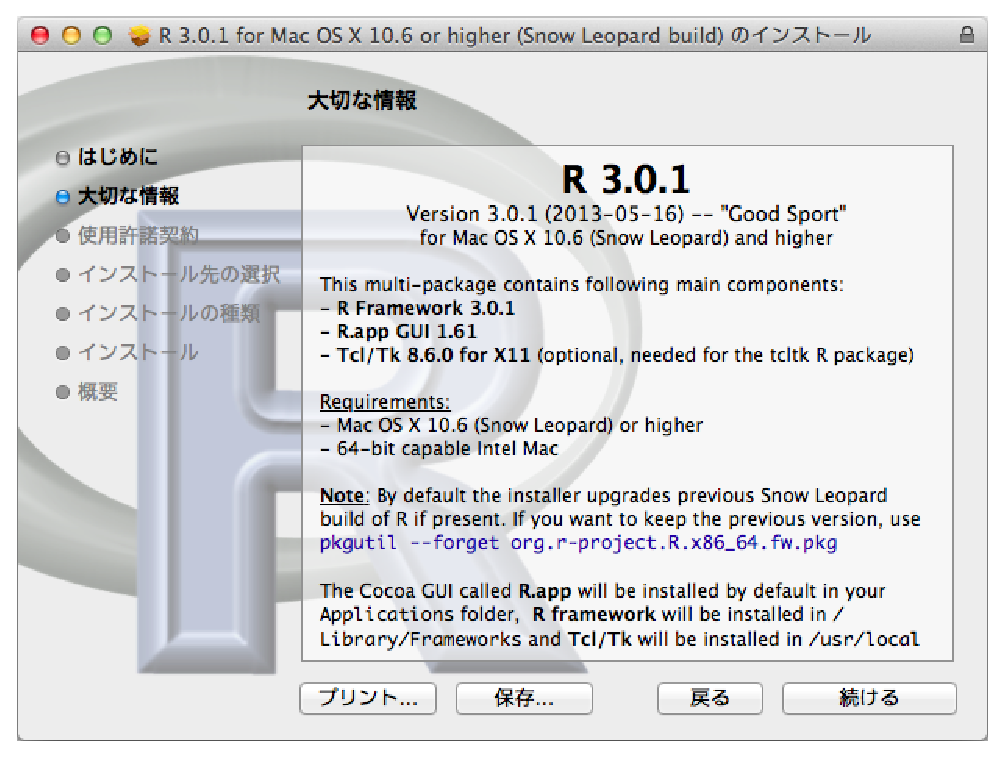
\includegraphics[width=8cm]{img/osx/osx003.eps} \\

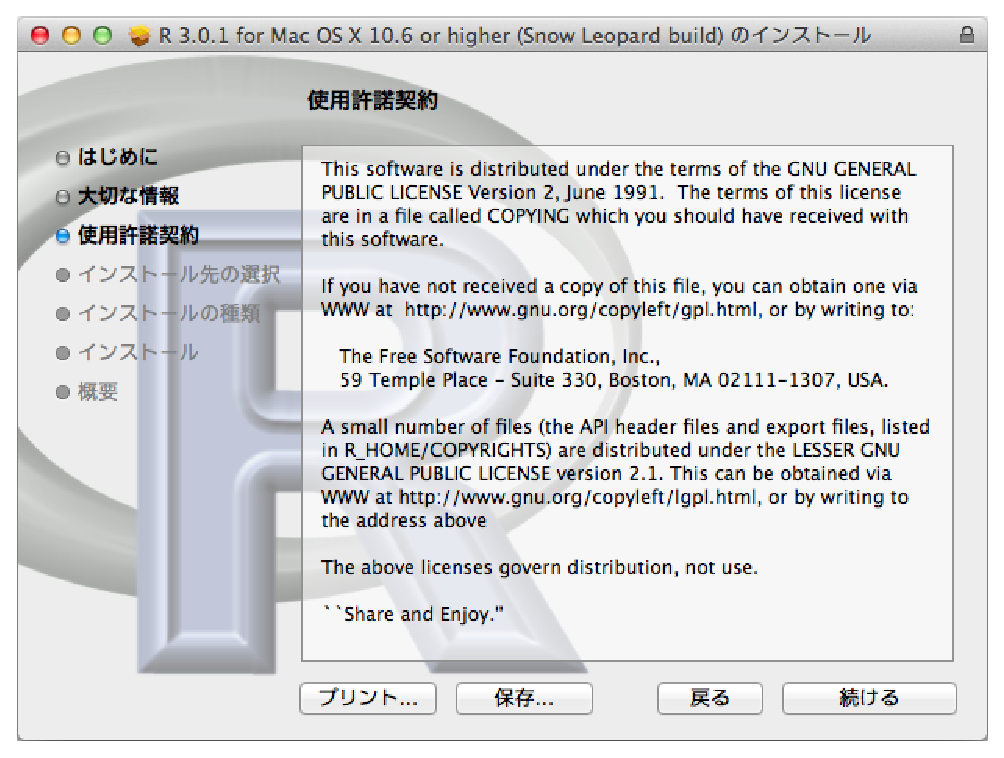
\includegraphics[width=8cm]{img/osx/osx004.eps}\hspace{0.8em} 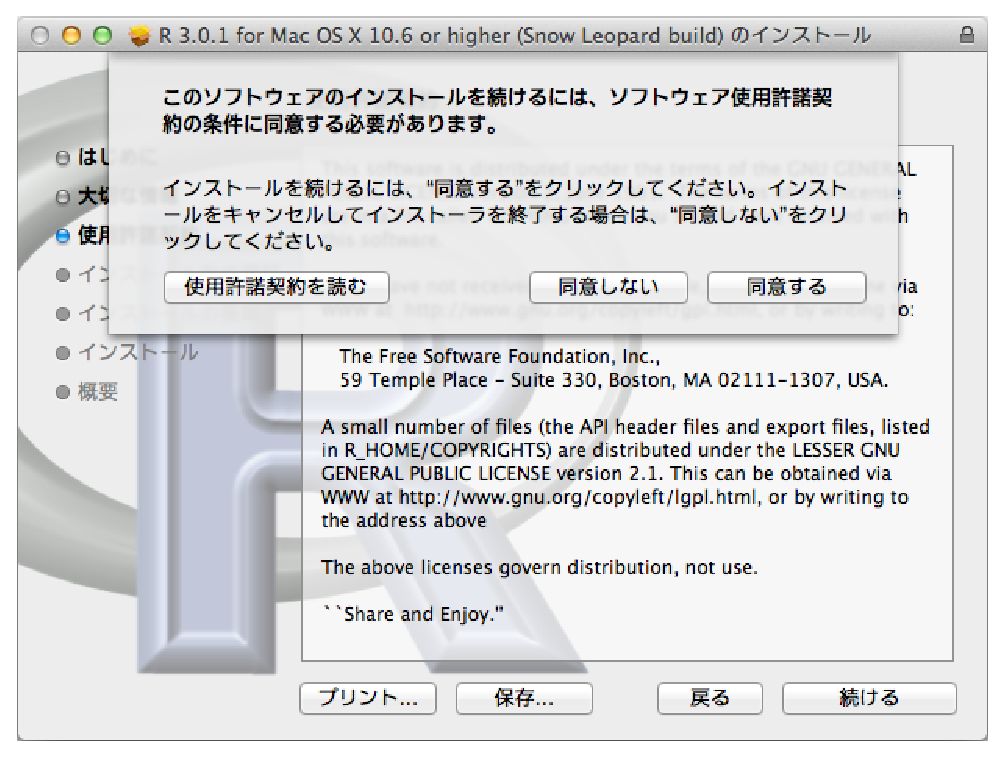
\includegraphics[width=8cm]{img/osx/osx005.eps}\\

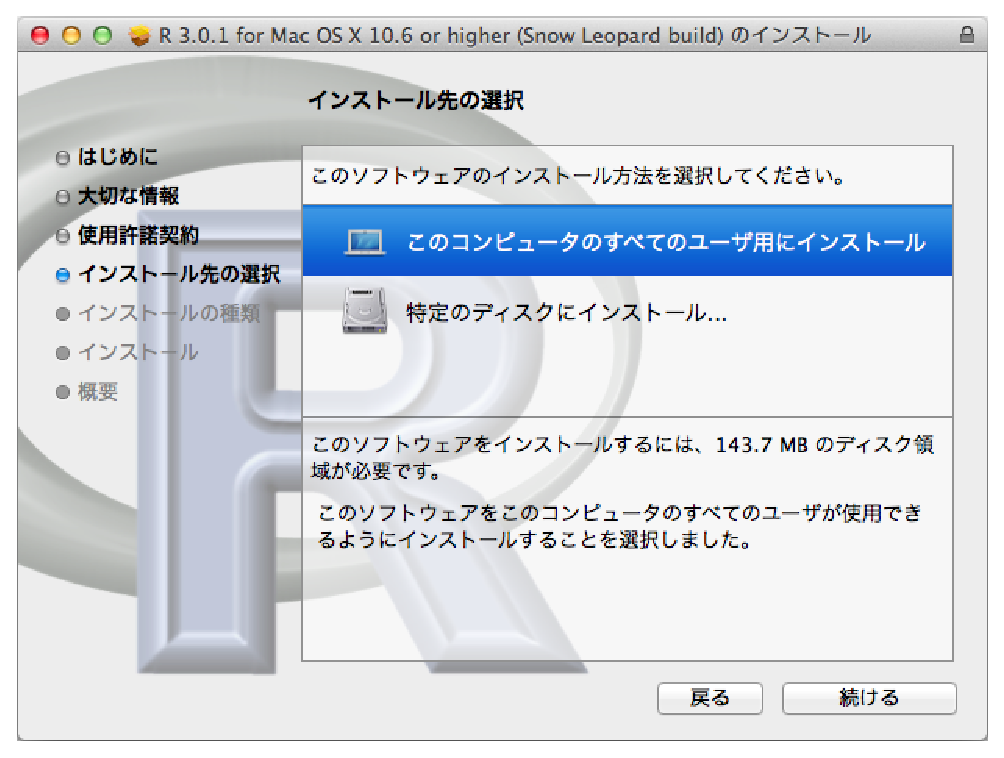
\includegraphics[width=8cm]{img/osx/osx006.eps}\hspace{0.8em} 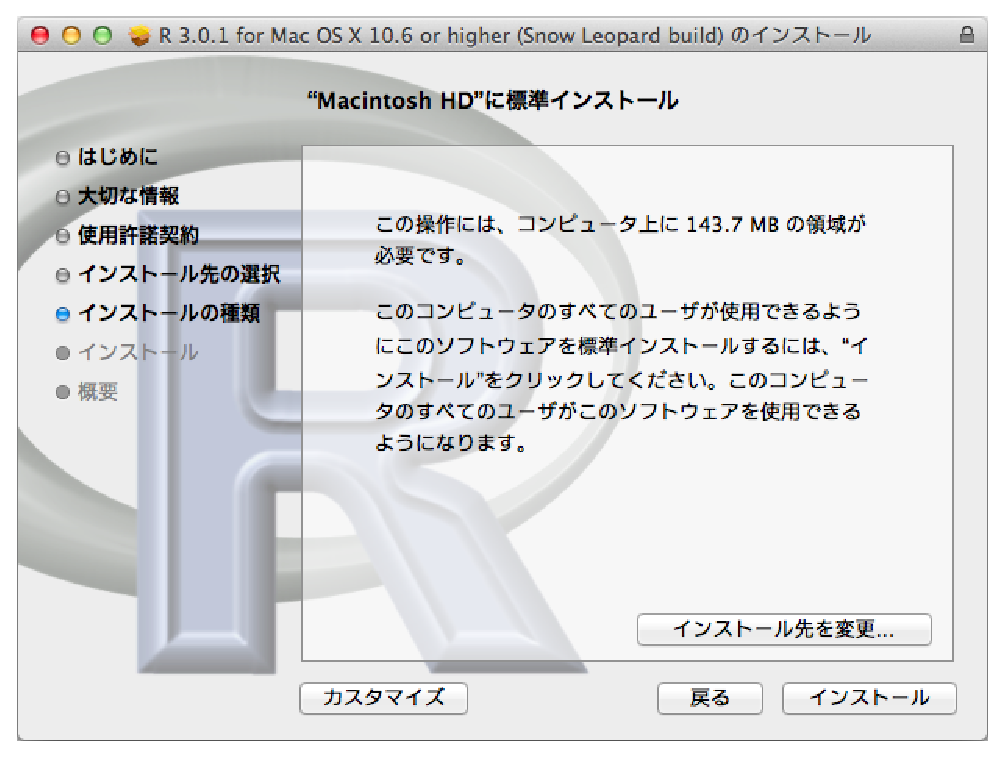
\includegraphics[width=8cm]{img/osx/osx007.eps}\\


\includegraphics[width=8cm]{img/osx/osx008.eps}\hspace{0.8em} 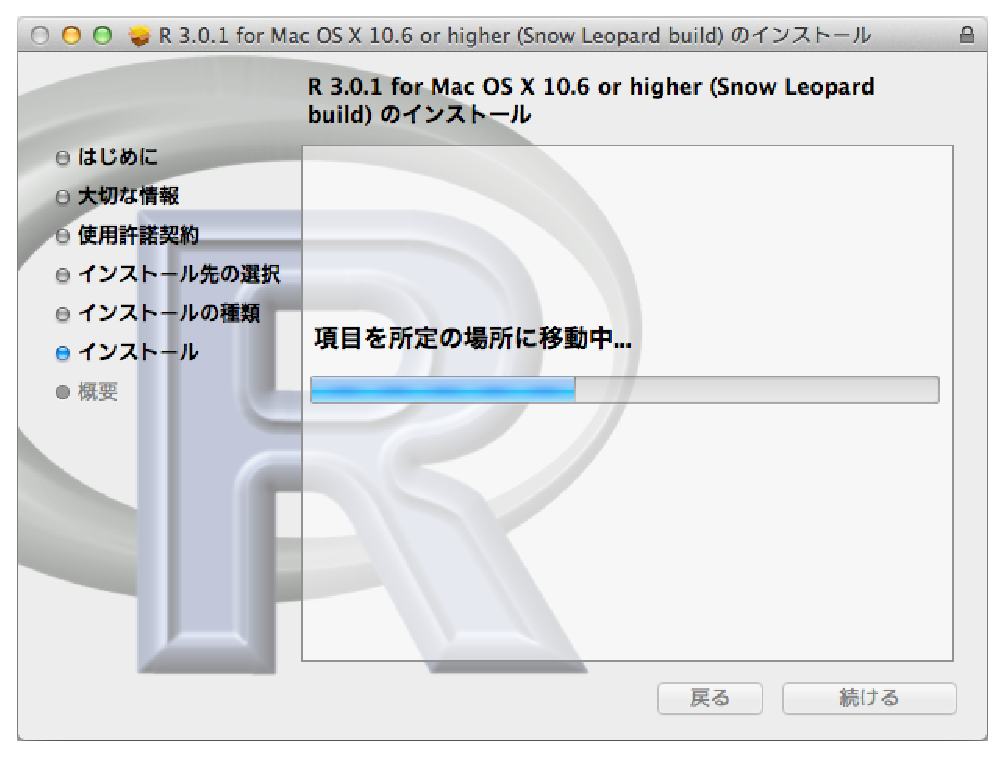
\includegraphics[width=8cm]{img/osx/osx009.eps}\\

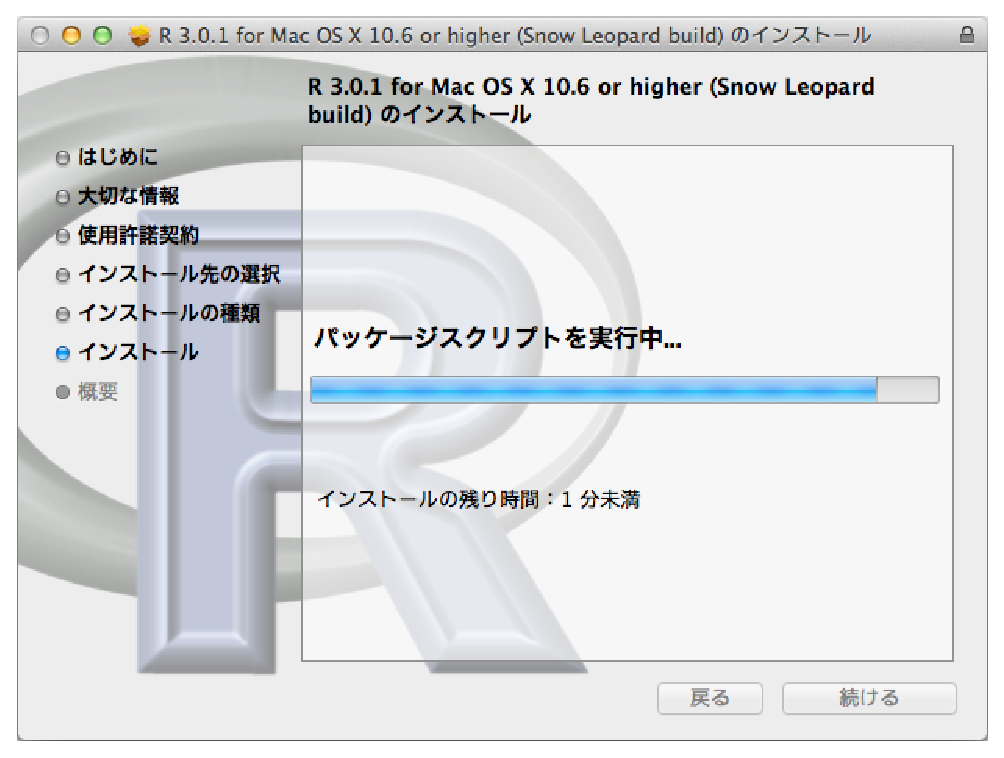
\includegraphics[width=8cm]{img/osx/osx010.eps}\hspace{0.8em} 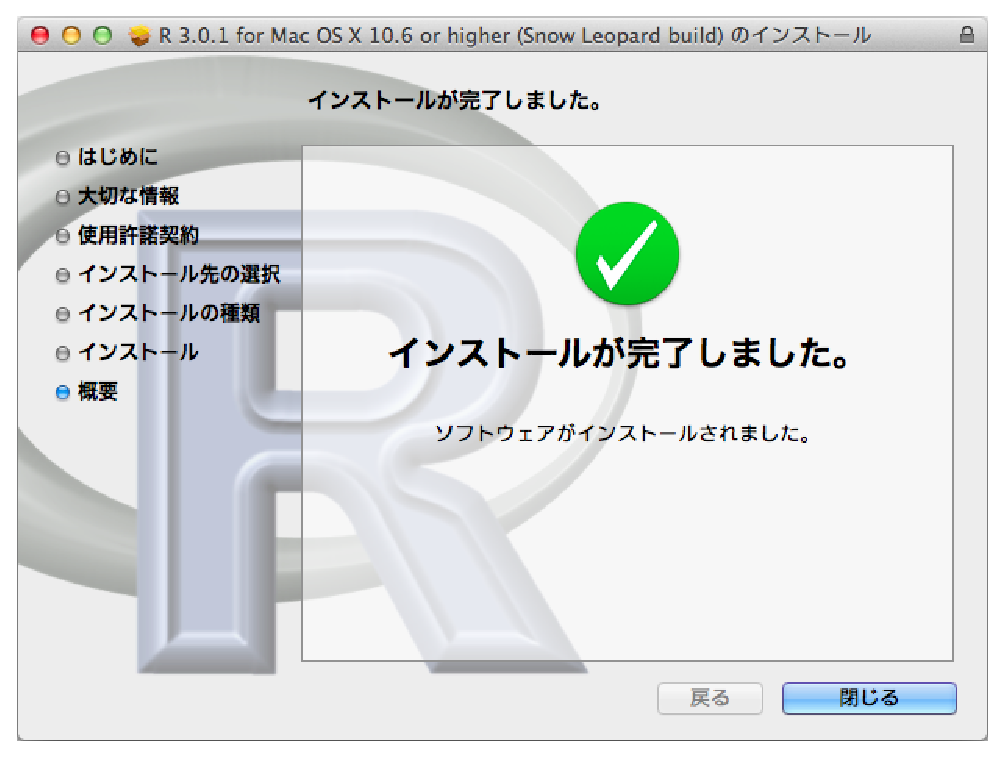
\includegraphics[width=8cm]{img/osx/osx011.eps}\\

以上でインストールは完了する.\\

アプリケーションにある 
\includegraphics[width=1.8cm]{img/osx/osx012.eps}より起動する.
\subsection{Linuxの場合}
パッケージ管理システムでインストールが可能.\verb+apt-get+では以下の様にインストールを行う.
\begin{breakbox}
\begin{verbatim}
sudo apt-get update
sudo apt-get install r-base
\end{verbatim}
\end{breakbox}
しかしながら,最新版への更新は遅めになるので,以下のように設定しても良い.
\verb+/etc/apt/sources.list+を管理者権限でで編集し
\begin{breakbox}
\begin{verbatim}
deb http://cran.ism.ac.jp/bin/linux/ubuntu precise/
\end{verbatim}
\end{breakbox}
を最終行に追記.
\begin{breakbox}
\begin{verbatim}
gpg --keyserver keyserver.ubuntu.com --recv-key E084DAB9
gpg -a --export E084DAB9 | sudo apt-key add -
sudo apt-get update
sudo apt-get install r-base
\end{verbatim}
\end{breakbox}
r-baseのレポジトリが標準のubuntuミラーではなくなりCRANのものになる.\\
細かい話は \url{http://www.trifields.jp/install-r-in-ubuntu-1000} や\\ \url{http://www.trifields.jp/how-to-deal-with-when-you-can-not-update-the-r-in-ubuntu-1515} あたりを参照してください.
\newpage
\section{基本的な計算}
\subsection{起動と使い方}
通常 \verb+>+ が表示されており,入力待ちの状態である.式や関数を入力しEnterを押せば計算結果が表示される.
\begin{breakbox}
\begin{verbatim}
> 1+2
[1] 3
> (1+2i)*(1-2i)
[1] 5+0i
> sum(1:10)
[1] 55
> rep(1,10)
[1] 1 1 1 1 1 1 1 1 1 1
> seq(1,5,0.5)
[1] 1.0 1.5 2.0 2.5 3.0 3.5 4.0 4.5 5.0
> ubuntu<-c(1,2,3,4,5,6)
> ubuntu
[1] 1 2 3 4 5 6
# コメントアウトは # です.
\end{verbatim}
\end{breakbox}
代入演算子は \verb+<-+,\verb+=+,\verb+->+ が用意されている.推奨は \verb+<-+ である.
\begin{description}
\item[四則演算の演算子]\mbox{}
\begin{table}[H]
\begin{center}
% \caption{表}
\vspace{1zw}
\label{03AB-A2}
\begin{tabular}{c|c}
\noalign{\hrule height 1pt}
演算子&意味\\ \hline
{\tt +}&足し算\\
\verb+^+&累乗\\
\verb+-+&引き算\\
\verb+%/%+&整数商\\
\verb+*+&掛け算\\
\verb+%%+&剰余\\
\verb+/+&割り算\\
\noalign{\hrule height 1pt}
\end{tabular}
\end{center}
\end{table}
\item[特殊な演算子]\mbox{}
\begin{table}[H]
\begin{center}
% \caption{表}
\vspace{1zw}
\label{03AB-A2}
\begin{tabular}{c|c}
\noalign{\hrule height 1pt}
演算子&意味\\ \hline
\verb+:+&公差$\pm$1の数列の作成\\
\verb+%*%+&行列積\\
\verb+%o%+&外積\\
\verb+[ ]+&配列や行列の要素の取出し\\
\verb+[[ ]]+&リスト成分の取出し\\
\verb+$+&データフレーム内の変数の取出し\\
\noalign{\hrule height 1pt}
\end{tabular}
\end{center}
\end{table}
\end{description}

オブジェクトの名前は予約語(すでに基本的な関数で使われている名前)でなければ使用できる.演算子を使うことや名前の最初に数字や\verb+_+(アンダーバー)を使うことはできない.必要であれば \verb+.+(ドット)か \verb+_+(アンダーバー) を使用する.ちなみに日本語も使用可能ではあるが,対応していないライブラリがあるので使用にはあまり適さない.
前に使った命令は入力時にキーボードの「↑」を押すと履歴をさかのぼることができる.
\begin{breakbox}
\begin{verbatim}
> 2*ubuntu
[1]  2  4  6  8 10 12
> 秋元="akimoto"
> 秋元
[1] "akimoto"
> debian=matrix(1:12,3,4)
> debian
     [,1] [,2] [,3] [,4]
[1,]    1    4    7   10
[2,]    2    5    8   11
[3,]    3    6    9   12
> matrix(1:12,3,4,byrow=T)
     [,1] [,2] [,3] [,4]
[1,]    1    2    3    4
[2,]    5    6    7    8
[3,]    9   10   11   12
> t(debian)
     [,1] [,2] [,3]
[1,]    1    2    3
[2,]    4    5    6
[3,]    7    8    9
[4,]   10   11   12
> debian*debian
     [,1] [,2] [,3] [,4]
[1,]    1   16   49  100
[2,]    4   25   64  121
[3,]    9   36   81  144
> debian%*%t(debian)
     [,1] [,2] [,3]
[1,]  166  188  210
[2,]  188  214  240
[3,]  210  240  270
> ubuntu[3]
[1] 3
> debian[2,]
[1]  2  5  8 11
> debian[,3]
[1] 7 8 9
> debian[2,3]
[1] 8
\end{verbatim}
\end{breakbox}

四則演算の演算子では,要素のそれぞれが計算され,行列の積は計算できない.

この{\tt matrix}関数では\verb+matrix(行列の要素,行の数,列の数,…)+というようにオプション引数が存在する.この引数を確認するには\verb+args(matrix)+と入力することで確認できる.
\begin{breakbox}
\begin{verbatim}
> args(matrix)
function (data = NA, nrow = 1, ncol = 1, byrow = FALSE, dimnames = NULL) 
NULL
\end{verbatim}
\end{breakbox}

{\tt args}関数を使用することで引数の名前がわかるが,引数の名前だけでは,必要な情報がそろわない場合がある.そのような場合は,ヘルプページを表示すればよい.
\begin{breakbox}
\begin{verbatim}
> ?matrix
starting httpd help server ... done
> help(matrix)
\end{verbatim}
\end{breakbox}

以下の,マニュアルが表示される.関数の説明や使い方,引数,例などが英語で記されている.
\begin{center}
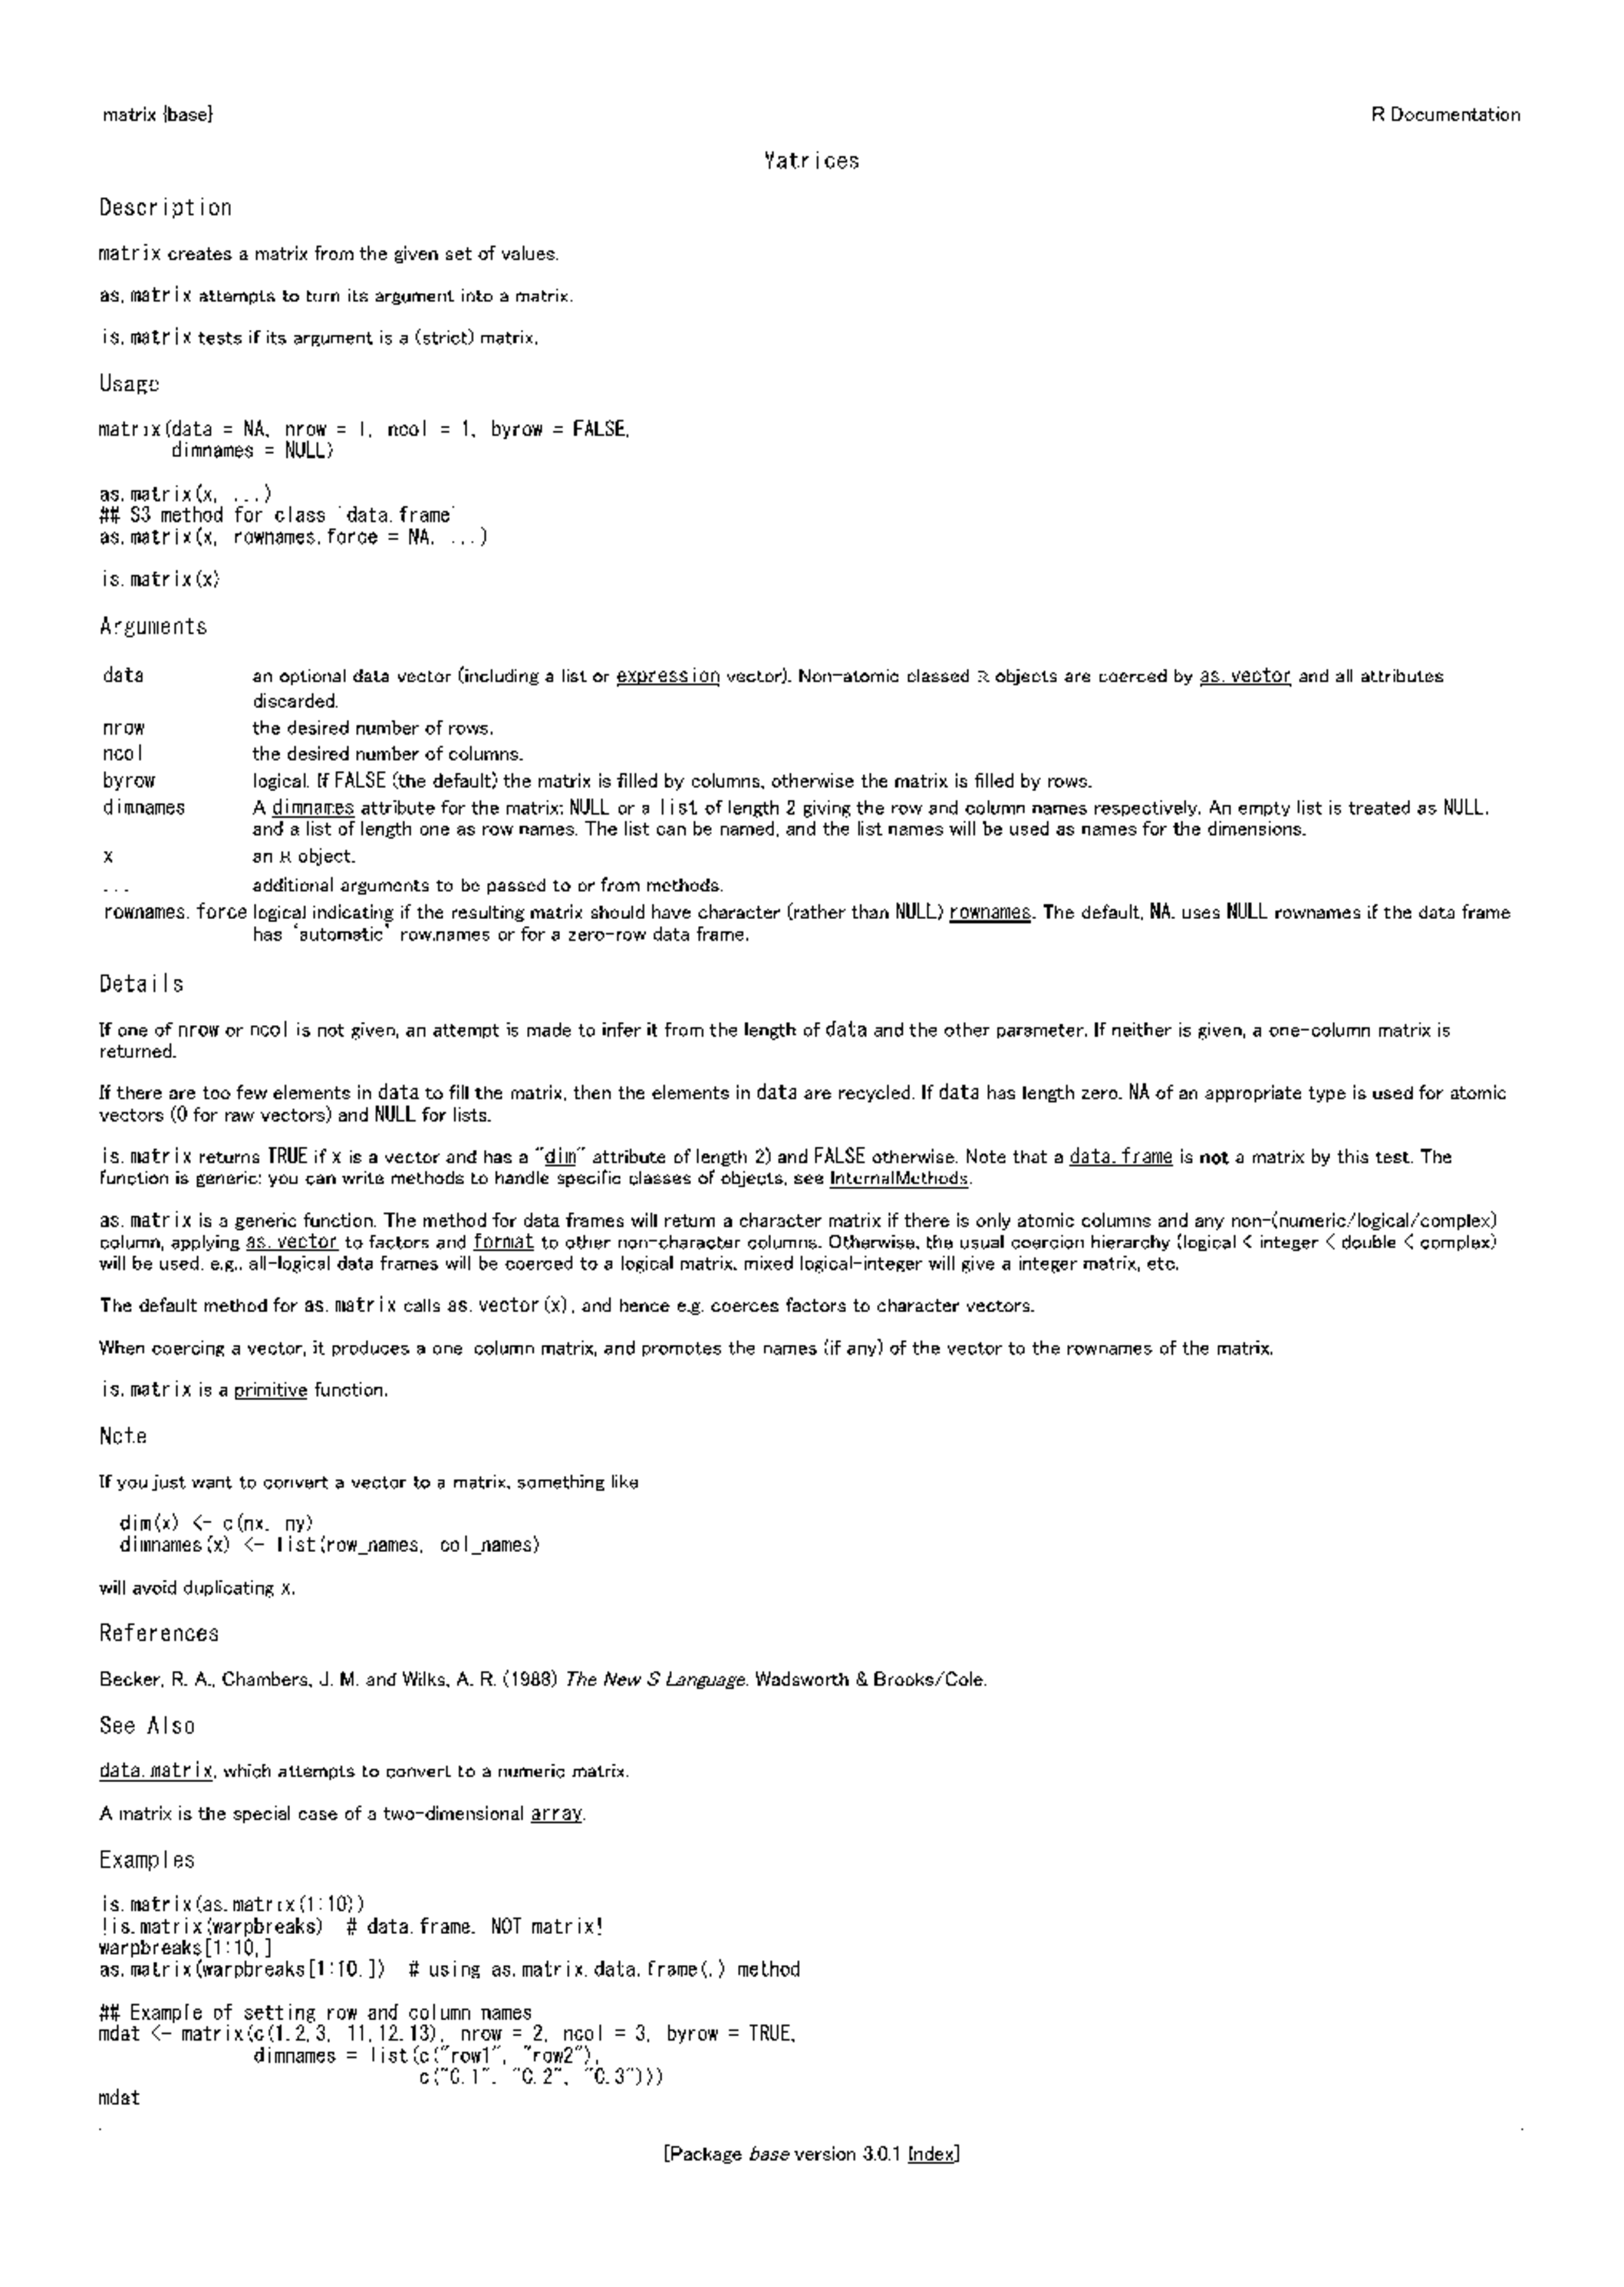
\includegraphics[height=15cm]{img/matrices.eps}
\end{center}

\subsection{オブジェクトの管理と設定}
\subsubsection{オブジェクトの型を変換する}
オブジェクトには様々な型やデータ構造がある.確認するには\verb+class(オブジェクト名)+や\verb+str(オブジェクト名)+などの関数での確認が必要な場合がある.
\begin{breakbox}
\begin{verbatim}
> class(iris)
[1] "data.frame"
> str(iris)
'data.frame':   150 obs. of  5 variables:
 $ Sepal.Length: num  5.1 4.9 4.7 4.6 5 5.4 4.6 5 4.4 4.9 ...
 $ Sepal.Width : num  3.5 3 3.2 3.1 3.6 3.9 3.4 3.4 2.9 3.1 ...
 $ Petal.Length: num  1.4 1.4 1.3 1.5 1.4 1.7 1.4 1.5 1.4 1.5 ...
 $ Petal.Width : num  0.2 0.2 0.2 0.2 0.2 0.4 0.3 0.2 0.2 0.1 ...
 $ Species     : Factor w/ 3 levels "setosa","versicolor",..: 1 1 1 1 1 1 1 1 1 1 ...
> iris$Petal.Length=as.factor(iris$Petal.Length)
> str(iris)
'data.frame':   150 obs. of  5 variables:
 $ Sepal.Length: num  5.1 4.9 4.7 4.6 5 5.4 4.6 5 4.4 4.9 ...
 $ Sepal.Width : num  3.5 3 3.2 3.1 3.6 3.9 3.4 3.4 2.9 3.1 ...
 $ Petal.Length: Factor w/ 43 levels "1","1.1","1.2",..: 5 5 4 6 5 8 5 6 5 6 ...
 $ Petal.Width : num  0.2 0.2 0.2 0.2 0.2 0.4 0.3 0.2 0.2 0.1 ...
 $ Species     : Factor w/ 3 levels "setosa","versicolor",..: 1 1 1 1 1 1 1 1 1 1 ...
\end{verbatim}
\end{breakbox}
このように型を変更することができる.
\begin{description}
\item[型の確認や変更の関数]\mbox{}
\begin{table}[H]
\begin{center}
% \caption{表}
\vspace{1zw}
\label{03AB-A2}
\begin{tabular}{c|l|l}
\noalign{\hrule height 1pt}
&\multicolumn{1}{l|}{型の確認}&\multicolumn{1}{c}{変換}\\ \hline
実数&\verb+is.numeric()+&\verb+as.numeric()+\\
整数&\verb+is.integer()+&\verb+as.integer()+\\
複素数&\verb+is.complex()+&\verb+as.complex()+\\
文字列&\verb+is.character()+&\verb+as.character()+\\
論理値&\verb+is.logical()+&\verb+as.logical()+\\
\noalign{\hrule height 1pt}
\end{tabular}
\end{center}
\end{table}
\item[データ構造の確認や変更の関数]\mbox{}
\begin{table}[H]
\begin{center}
% \caption{表}
\vspace{1zw}
\label{03AB-A2}
\begin{tabular}{c|l|l}
\noalign{\hrule height 1pt}
&\multicolumn{1}{c|}{構造の確認}&\multicolumn{1}{c}{変換}\\ \hline
ベクトル&\verb+is.vector()+&\verb+as.vector()+\\
行列&\verb+is.matrix()+&\verb+as.matrix()+\\
配列&\verb+is.array()+&\verb+as.array()+\\
リスト&\verb+is.list()+&\verb+as.list()+\\
データフレーム&\verb+is.data.frame()+&\verb+as.data.frame()+\\
順序なし因子&\verb+is.factor()+&\verb+as.factor()+\\
順序つき因子&\verb+is.ordered()+&\verb+as.ordered()+\\
\noalign{\hrule height 1pt}
\end{tabular}
\end{center}
\end{table}
\end{description}

これらの{\tt is}で始まる関数は,{\tt TRUE や FALSE}を返す.また,データの内容を確認したい場合は{\tt head}関数や{\tt tail}関数を使用する.この関数はデータの上から,もしくは下から6つ分のデータを表示する関数である.
\begin{breakbox}
\begin{verbatim}
> head(iris)
  Sepal.Length Sepal.Width Petal.Length Petal.Width Species
1          5.1         3.5          1.4         0.2  setosa
2          4.9         3.0          1.4         0.2  setosa
3          4.7         3.2          1.3         0.2  setosa
4          4.6         3.1          1.5         0.2  setosa
5          5.0         3.6          1.4         0.2  setosa
6          5.4         3.9          1.7         0.4  setosa
> tail(iris)
    Sepal.Length Sepal.Width Petal.Length Petal.Width   Species
145          6.7         3.3          5.7         2.5 virginica
146          6.7         3.0          5.2         2.3 virginica
147          6.3         2.5          5.0         1.9 virginica
148          6.5         3.0          5.2         2.0 virginica
149          6.2         3.4          5.4         2.3 virginica
150          5.9         3.0          5.1         1.8 virginica
\end{verbatim}
\end{breakbox}
\subsubsection{データの中の変数を呼び出す}
前述のとおりデータの中の変数を使う場合には\verb+data$var+というような使い方を書いたが,実際には指定することが面倒になる場合がある.その場合,{\tt attach}関数を用いてそのまま変数を使用することができる.
\begin{breakbox}
\begin{verbatim}
> head(Sepal.Length)
 以下にエラー head(Sepal.Length) :  オブジェクト 'Sepal.Length' がありません 
> attach(iris)
> head(Sepal.Length)
[1] 5.1 4.9 4.7 4.6 5.0 5.4
\end{verbatim}
\end{breakbox}
使い終わったら,{\tt detach}関数で解除することをお奨めする.
\begin{breakbox}
\begin{verbatim}
> detach(iris)
> head(Sepal.Length)
 以下にエラー head(Sepal.Length) :  オブジェクト 'Sepal.Length' がありません 
\end{verbatim}
\end{breakbox}
\subsubsection{作成したオブジェクトの削除}
続けて使用しているとオブジェクトが不必要になることがある.その場合,オブジェクトを消去すればよい.
\begin{breakbox}
\begin{verbatim}
> ls()
[1] "chuo"   "debian" "ubuntu"
> objects()
[1] "chuo"   "debian" "ubuntu"
> rm(debian)
> ls()
[1] "chuo"   "ubuntu"
> rm(list=ls(all=TRUE))
> ls()
character(0)
\end{verbatim}
\end{breakbox}
{\tt ls}関数や{\tt objects}関数でオブジェクトを確認できる.{\tt rm}関数で個別に消去もでき,全消去することもできる.また,メニューより全消去することも可能だ.

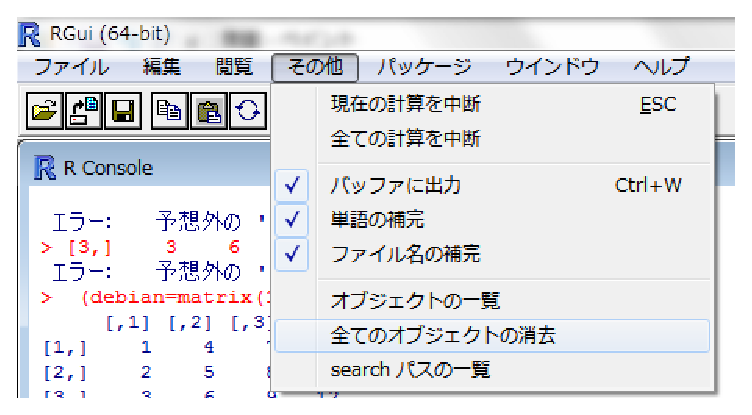
\includegraphics[height=4cm]{img/windows/rmall.eps}\hspace{0.8em} 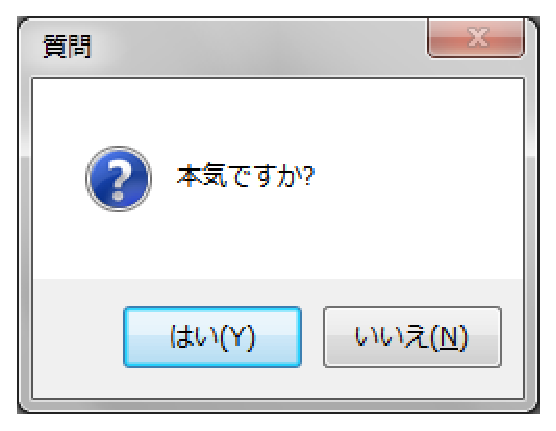
\includegraphics[height=4cm]{img/windows/honki.eps}
\subsection{基本的な関数}
ここでは,主に使用する関数を一部抜粋して記す.
\begin{table}[H]
\begin{center}
% \caption{表}
\vspace{1zw}
\begin{tabular}{l|l}
\noalign{\hrule height 1pt}
\multicolumn{1}{c|}{関 数}&\multicolumn{1}{c}{種 類}\\ \hline
\verb+c(x1,x2,...)+ &配列(ベクトルの作成)\\
\rowcolor{bl} \verb+rep(x,times)+ &{\tt x}を{\tt times}回繰り返す\\
\verb+seq(初項,末項,公差)+ &等差数列の作成\\
\rowcolor{bl} \verb+matrix(c(x1,x2,...),行数,列数,byrow=FALSE)+ &行列の作成 ({\tt byrow}は配列を列方向に代入する引数)\\
\verb+abs(x)+ &絶対値\\
\rowcolor{bl} \verb+mean(x)+ &平均\\
\verb+var(x)+ &分散\\
\rowcolor{bl} \verb+median(x)+ &中央値\\
\verb+max(x)+ &最大値\\
\rowcolor{bl} \verb+min(x)+ &最小値\\
\verb+cor(x,y)+ &相関係数\\
\rowcolor{bl} \verb+t()+&行列の転置\\
\verb+solve(x)+&逆行列の生成\\
\rowcolor{bl} \verb+eigen(x)+ &固有値と固有ベクトル\\
\verb+sqrt(x)+ &平方根\\
\rowcolor{bl} \verb+exp(x)+ &指数関数\\
\verb+log(x,base=exp(1))+ &{\tt base}を底とした対数\\
\rowcolor{bl} \verb+sum(x)+ &総和\\
\verb+cumsum(x)+ &累積和\\
\rowcolor{bl} \verb+prod(x)+ &総乗\\
\verb+cumprod(x)+ &累積積\\
\rowcolor{bl} \verb+sin(x)+ &正弦関数\\
\verb+floor(x)+ &切り捨て\\
\rowcolor{bl} \verb+ceiling(x)+ &切り上げ\\
\verb+round(x, digits = 0)+ &整数に丸める\\
\rowcolor{bl} \verb+length(x)+ &ベクトルの長さを調べる\\
\verb+dim(x)+ &行列やデータフレームの行数と列数を調べる\\
\noalign{\hrule height 1pt}
\end{tabular}
\end{center}
\end{table}
引数に数値やベクトル,行列を入れることによって計算結果を得ることができる.1つの数値を入力する関数にベクトルや行列を代入すると,Rでは要素ごとに計算を行う.
\subsubsection{確率分布}
Rでは乱数発生アルゴリズムが存在する.併せて確率密度関数や累積分布関数の計算もできるので覚えておくとよい.
\begin{table}[H]
\begin{center}
% \caption{表}
\vspace{1zw}
\begin{tabular}{l|l}
\noalign{\hrule height 1pt}
\multicolumn{1}{c|}{種類}&\multicolumn{1}{c}{関数}\\ \hline
確率密度関数&{\tt d*(確率点)}\\
累積分布関数&{\tt p*(確率点)}\\
確率点(累積分布関数の逆関数)&{\tt q*(確率)}\\
乱数発生&{\tt r*(個数)}\\
\noalign{\hrule height 1pt}
\end{tabular}
\end{center}
\end{table}

以下では主な確率分布を取り上げる.引数に初期値が設定されているものもある.
\begin{table}[H]
\begin{center}
% \caption{表}
\vspace{1zw}
\begin{tabular}{l||l|l}
\noalign{\hrule height 1pt}
\multicolumn{1}{c||}{確率分布}&\multicolumn{1}{c|}{関数}&\multicolumn{1}{c}{引数}\\ \hline
一様分布&{\tt unif}&{\tt min=0,max=1}\\
二項分布&{\tt binom}&{\tt size, prob}\\
正規分布&{\tt norm}&{\tt mean=0,sd=1}\\
ポアソン分布&{\tt pois}&{\tt lambda}\\
指数分布&{\tt exp}&{\tt rate=1}\\
$\chi^2$分布&{\tt chisq}&{\tt df,ncp=0}\\
\noalign{\hrule height 1pt}
\end{tabular}
\end{center}
\end{table}

つまり,一様分布$U(0,1)$において,$P(X=0.5)$の確率を求めたい場合は\verb+dunif(0.5)+,$P(X<0.5)$を求めたい場合は\verb+punif(0.5)+,$P(X<y)=0.5$となる$y$を求める場合は\verb+qunif(0.5)+,この一様分布に従う乱数を10個生成したい場合は\verb+runif(10)+となる.
\subsection{作図}
ここでは,{\tt plot}関数を用いて作図を行う.\\
基本形は{\tt plot(x,y)}もしくは{\tt plot(y\verb+~+x)}である.変数が一つでもよい.オプション引数を特に指定しない場合は,自動で適当な作図してくれる.
\begin{screen}
\verb+plot(x,y,type="",xlab="",ylab="",main="",sub="",xlim=c(,),ylim=c(),axes=TRUE,pch="",+\\
\verb+col="",lty="",lwd="")+ 
\end{screen}
引数を指定しない場合は自動で初期値となる.
\subsubsection{軸}
\begin{description}
\item[軸の表示] \mbox{}\\
{\tt axes=FALSE}とした場合,図の枠や軸は表示されない.\\
その場合,あとから{\tt box()}関数で枠を書くことができる.
\begin{screen}
{\tt box()}
\end{screen}
後から軸を書く場合は,{\tt axis()}関数を使用する.
\begin{screen}
\begin{verbatim}
axis(1) # 下の軸を表示する 2:左,3:上,4:右
axis(1,at=c(0.4,0.6,0.9)) # 引数 at を用いて軸の任意の箇所に数字を表示することも可能だ.
\end{verbatim}
\end{screen}
\item[表題] \mbox{}\\
表題は{\tt main},サブタイトルは{\tt sub}で指定する.文字列は\verb+""+で指定すること.作図後に表題を追加する場合は{\tt title()}関数を使用する.
\begin{screen}
\begin{verbatim}
title(main="表題",sub="サブタイトル")
\end{verbatim}
\end{screen}
\item[X軸,Y軸の名前] \mbox{}\\
{\tt xlab}と{\tt ylab}で指定する.同様に,後から追加する場合は{\tt title}関数を使用する.
\begin{screen}
\begin{verbatim}
title(xlab="X軸の名前",ylab="Y軸の名前")
\end{verbatim}
\end{screen}
\item[X軸,Y軸の上限と下限] \mbox{}\\
{\tt xlim=c(上限,下限)},{\tt ylim=c(上限,下限)}で指定する.
\end{description}
\subsubsection{種類}
{\tt type}で指定する.以下はRの標準で用意されているグラフの一覧である.
\begin{table}[H]
\begin{center}
% \caption{表}
\vspace{1zw}
\label{03AB-A2}
\begin{tabular}{c|l}
\noalign{\hrule height 1pt}
指定&\multicolumn{1}{c}{種類}\\ \hline
\verb+type="p"+ &点プロット(2変数でのデフォルト)\\
\verb+type="l"+ &線プロット(折れ線グラフ・1変数でのデフォルト)\\
\verb+type="b"+ &点と線のプロット\\
\verb+type="c"+ &\verb+"b"+ において点を描かないプロット\\
\verb+type="o"+ &点プロットと線プロットの重ね書き\\
\verb+type="h"+ &各点からx 軸までの垂線プロット\\
\verb+type="s"+ &左側の値にもとづいて階段状に結ぶ\\
\verb+type="S"+ &右側の値にもとづいて階段状に結ぶ\\
\verb+type="n"+ &軸だけ描いてプロットしない(続けて低水準関数でプロットする場合)\\
\noalign{\hrule height 1pt}
\end{tabular}
\end{center}
\end{table}

また,点をプロットする場合プロット記号を指定することができる.\verb+pch+で指定する.
\begin{center}
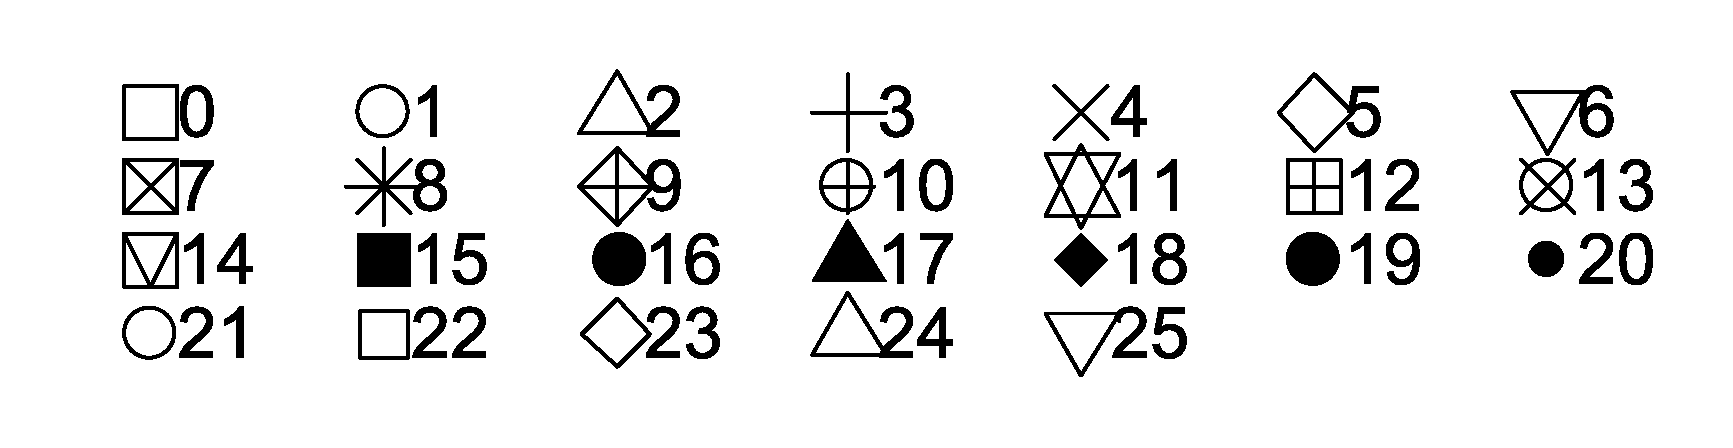
\includegraphics[height=2cm]{img/pch.eps}
\end{center}

なお,プロット記号の大きさは,\verb+cex+で指定する.線をプロットする場合,線の種類({\tt lty})や線の幅({\tt lwd})を指定することができる.
\begin{figure}[H]
  \begin{center}
    \begin{tabular}{c}
      % 1
      \begin{minipage}{0.3\hsize}
        \begin{center}
          \verb+lty+で線の種類の指定\\
          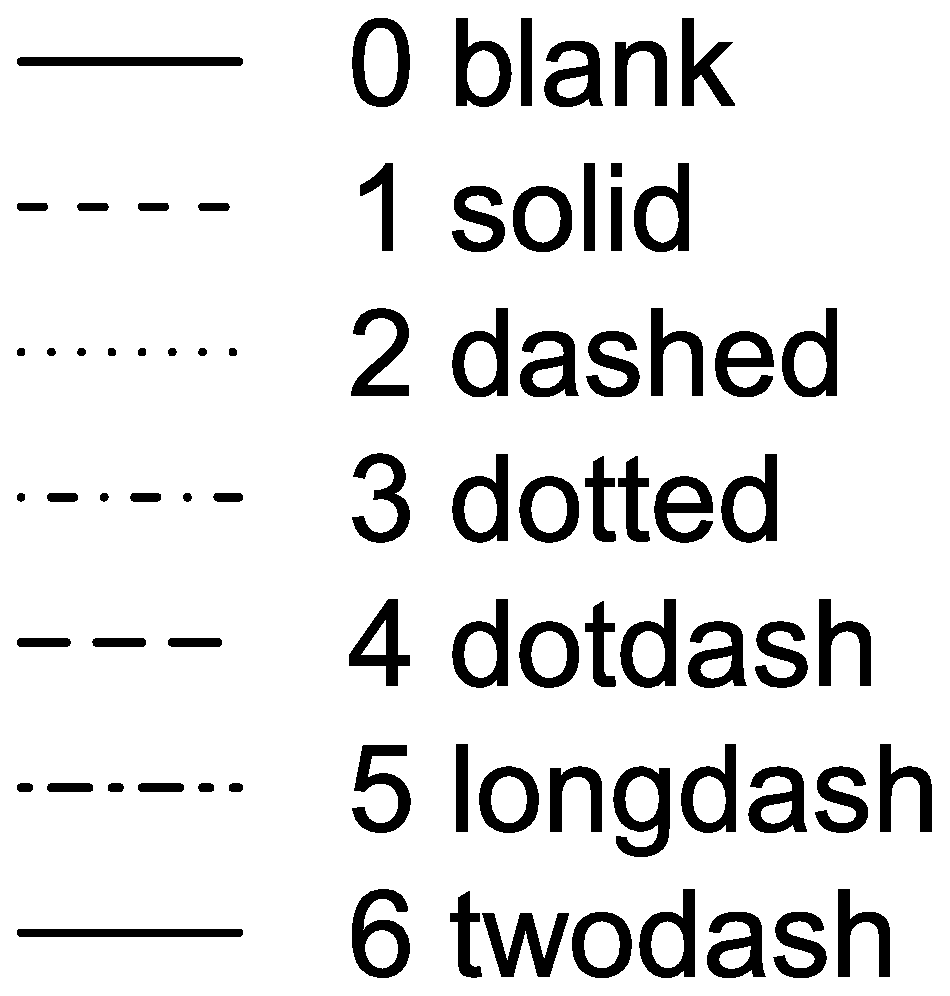
\includegraphics[height=2.5cm]{img/lty.eps}
        \end{center}
      \end{minipage}
      % 2
      \begin{minipage}{0.3\hsize}
        \begin{center}
          \verb+lwd+で線の太さの指定\\
          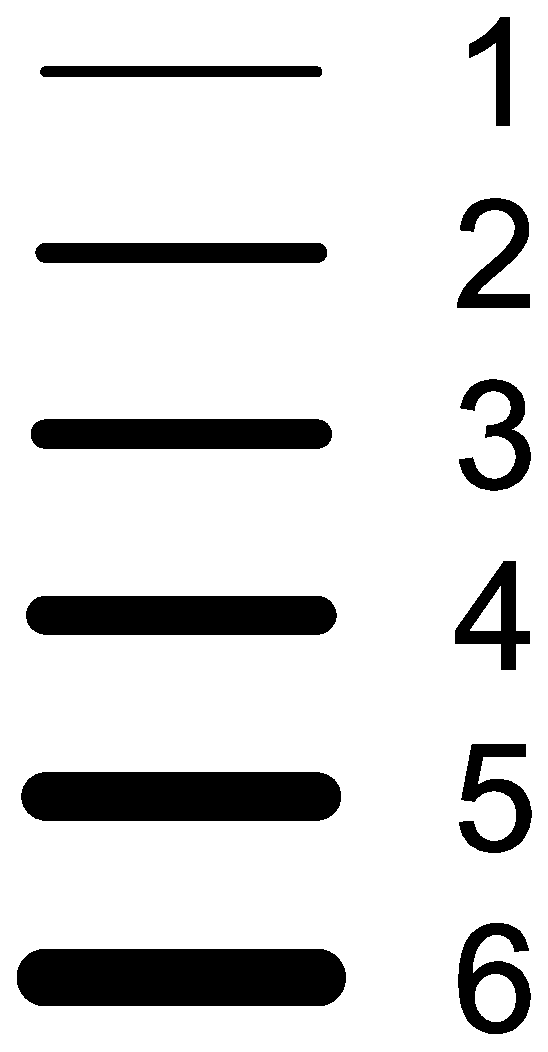
\includegraphics[height=2.5cm]{img/lwd.eps}
        \end{center}
      \end{minipage}
    \end{tabular}
  \end{center}
\end{figure}

他にも,色を変えることもできる.
\begin{table}[H]
\begin{center}
% \caption{表}
\vspace{1zw}
\label{03AB-A2}
\begin{tabular}{c||c|l}
\noalign{\hrule height 1pt}
色&番号&\multicolumn{1}{c}{名前}\\ \hline
■&\tt 1&\tt black\\
\textcolor{myred}{■}&\tt 2&\tt red\\
\textcolor{mygreen}{■}&\tt 3&\tt green\\
\textcolor{myblue}{■}&\tt 4&\tt blue\\
\textcolor{mycyan}{■}&\tt 5&\tt cyan\\
\textcolor{mymagenta}{■}&\tt 6&\tt magenta\\
\textcolor{myyellow}{■}&\tt 7&\tt yellow\\
\noalign{\hrule height 1pt}
\end{tabular}
\end{center}
\end{table}

16進数でRGBを指定することや,\verb+colors()+関数を使用して,Rに定義されている657色を選択することも可能である.
\begin{breakbox}
\begin{verbatim}
> head(colors())
[1] "white"         "aliceblue"     "antiquewhite"  "antiquewhite1"
[5] "antiquewhite2" "antiquewhite3"
> plot(lynx,col=colors()[25])
> plot(lynx,col="#8080FF")
\end{verbatim}
\end{breakbox}
{\tt pch}や{\tt col}に\verb+c(1,1,2,1,1)+と指定すれば,任意の箇所だけを色を変えたり,記号を変えることもできる.\\
また,{\tt lines()}や{\tt points()},{\tt abline()}関数を使用して,先ほどのプロットに点や線を重ねて書くこともできる.
\begin{screen}
\begin{verbatim}
abline(v=15) # x=15 に縦の直線を引く
abline(h=20,col=2) # y=20に横の直線を引く
\end{verbatim}
\end{screen}

Windows では表示されたグラフを右クリックすることで保存することや Microsoft Office Word に貼り付けることができる.




\noindent
{\bf \large{Macでの作図}}

Macで作図をする場合,文字が□に化けてしまう.そのため作図前に{\tt par}関数を用いて設定を変更するか,
\begin{screen}
\begin{verbatim}
par(family="HiraKakuProN-W3").
\end{verbatim}
\end{screen}
\verb+~/.Rprofile+を作成する必要がある.
\begin{screen}
\begin{verbatim}
setHook(packageEvent("grDevices", "onLoad"),
	function(...){
        if(.Platform$OS.type == "windows")
            grDevices::windowsFonts(sans ="MS Gothic",
                                    serif="MS Mincho",
                                    mono ="FixedFont")
        if(capabilities("aqua"))
            grDevices::quartzFonts(
              sans =grDevices::quartzFont(
                c("Hiragino Kaku Gothic Pro W3",
                  "Hiragino Kaku Gothic Pro W6",
                  "Hiragino Kaku Gothic Pro W3",
                  "Hiragino Kaku Gothic Pro W6")),
              serif=grDevices::quartzFont(
                c("Hiragino Mincho Pro W3",
                  "Hiragino Mincho Pro W6",
                  "Hiragino Mincho Pro W3",
                  "Hiragino Mincho Pro W6")))
        if(capabilities("X11"))
            grDevices::X11.options(
                fonts=c("-kochi-gothic-%s-%s-*-*-%d-*-*-*-*-*-*-*",
                        "-adobe-symbol-medium-r-*-*-%d-*-*-*-*-*-*-*"))
        grDevices::pdf.options(family="Japan1GothicBBB")
        grDevices::ps.options(family="Japan1GothicBBB")
        }
)

attach(NULL, name = "JapanEnv")
assign("familyset_hook",
       function() {
            winfontdevs=c("windows","win.metafile",
                          "png","bmp","jpeg","tiff")
            macfontdevs=c("quartz","quartz_off_screen")
            devname=strsplit(names(dev.cur()),":")[[1L]][1]
            if ((.Platform$OS.type == "windows") &&
                (devname %in% winfontdevs))
                    par(family="sans")
            if (capabilities("aqua") &&
                devname %in% macfontdevs)
                    par(family="sans")
       },
       pos="JapanEnv")
setHook("plot.new", get("familyset_hook", pos="JapanEnv"))
setHook("persp", get("familyset_hook", pos="JapanEnv"))
\end{verbatim}
\end{screen}
\subsection{関数の定義}
基本的な形式はこの形である.(入力した引数を)演算子し,{\tt return()}で返す.
\begin{screen}
\begin{verbatim}
myfunc<-function(x){
  a=x%%2
  return(a)
  }
\end{verbatim}
\end{screen}
\subsubsection{条件分岐(if文)}
\begin{screen}
\begin{verbatim}
myfunc<-function(x){
  a=x%%2
  if(a==0){
    return(TRUE) # a==0 が真の場合の処理
    }else if(a==1){
    return(FALSE) # a==0 が偽の場合で a==1 が真の場合の処理
    }else{
    return("Not Integer") # a==0 が偽の場合で a==1 が偽の場合の処理
    }
  }
\end{verbatim}
\end{screen}
この定義した関数で計算した結果が以下である.
\begin{breakbox}
\begin{verbatim}
> myfunc(1)
[1] FALSE
> myfunc(2)
[1] TRUE
> myfunc(2.1)
[1] "Not Integer"
\end{verbatim}
\end{breakbox}

なお,比較演算子や論理演算子は以下である.
\begin{description}
\item[比較演算子]\mbox{}
\begin{center}
\begin{tabular}{c|c}
\noalign{\hrule height 1pt}
演算子&\multicolumn{1}{c}{意味}\\ \hline
\verb+==+&$=$\\
\verb+!=+&$\ne$\\
\verb+>+&$>$\\
\verb+<+&$<$\\
\verb+>=+&$\geq$\\
\verb+<=+&$\leq$\\
\noalign{\hrule height 1pt}
\end{tabular}
\end{center}
\item[論理演算子]\mbox{}
\begin{center}
\begin{tabular}{c|lc}
\noalign{\hrule height 1pt}
演算子&\multicolumn{2}{c}{意味}\\ \hline
\verb+!+&否定&$\lnot$\\
\verb+&&+&論理積(かつ) &$ \land $ \\
\verb+||+&論理和(または) &$ \lor $ \\
\verb+xor()+&排他的論理和 &$\oplus$ \\
\noalign{\hrule height 1pt}
\end{tabular}
\end{center}
\end{description}

以下のように,比較演算だけを行うこともできる.また,ベクトルで演算を行えばベクトルの要素ごとの演算結果を返してくれる.
\begin{breakbox}
\begin{verbatim}
> 2==3
[1] FALSE
> 2==3||5==5
[1] TRUE
> c(1,2,3)!=c(3,2,1)
[1]  TRUE FALSE  TRUE
\end{verbatim}
\end{breakbox}

また,オブジェクトから条件に合うものだけを抽出したり,条件に合うオブジェクト内の要素の番号を得ることもできる.
\begin{breakbox}
\begin{verbatim}
> b=11:30
> b[b%%2==0] # bを2で割った余りが0の要素を表示
 [1] 12 14 16 18 20 22 24 26 28 30
> which(b%%2==0) # bを2で割った余りが0の要素の番号を表示
 [1]  2  4  6  8 10 12 14 16 18 20
\end{verbatim}
\end{breakbox}
\subsubsection{繰り返し(for分とwhile文)}
\begin{screen}
\begin{verbatim}
for(i in 1:10){
  #関数
  print(i)
  }
# 1:10ではなく任意のベクトルにしてもよい.
# この場合 i を変数として使える.

while (x <= 5) { # while ( 条件式 )
  x <- x + 1
  # 条件式が TRUE である限り式が繰り返される
  } 

\end{verbatim}
\end{screen}
\subsection{パッケージの利用}
前述のとおり,Rには多くのパッケージが存在している.パッケージを使用することで,解析手法や関数を導入することができる.
\begin{breakbox}
\begin{verbatim}
> install.packages("ismev") # ライブラリのインストール
 パッケージを 'C:/Users/User/Documents/R/win-library/2.15' 中にインストールします 
 ('lib' が指定されていないので) 
 --- このセッションで使うために,CRANのミラーサイトを選んでください --- 
 URL 'http://cran.rstudio.com/bin/windows/contrib/2.15/ismev_1.39.zip' を試しています 
Content type 'application/zip' length 192211 bytes (187 Kb)
 開かれた URL 
downloaded 187 Kb

 パッケージ 'ismev' は無事に展開され,MD5 サムもチェックされました 

 ダウンロードされたパッケージは,以下にあります 
        C:\Users\User\AppData\Local\Temp\Rtmp2BJBEa\downloaded_packages 
\end{verbatim}
\end{breakbox}
これで,パッケージのインストールは完了した.メニューより選択してインストールすることも可能だ.

インストールしたパッケージを呼び出すには,\verb+library+関数を使用する.
\begin{breakbox}
\begin{verbatim}
> library(ismev) # ライブラリの呼び出し
 要求されたパッケージ mgcv をロード中です 
This is mgcv 1.7-18. For overview type 'help("mgcv-package")'.
 警告メッセージ: 
 パッケージ ''ismev'' はバージョン 2.15.3 の R の下で造られました 
\end{verbatim}
\end{breakbox}
またコマンドではなくメニューからパッケージをインストールする方法もある.
\begin{figure}[H]
  \begin{center}
    \begin{tabular}{c}
      % 1
      \begin{minipage}{0.4\hsize}
        %\begin{center}
          メニューの``パッケージ"から\\``パッケージのインストール"を選択し,\\
          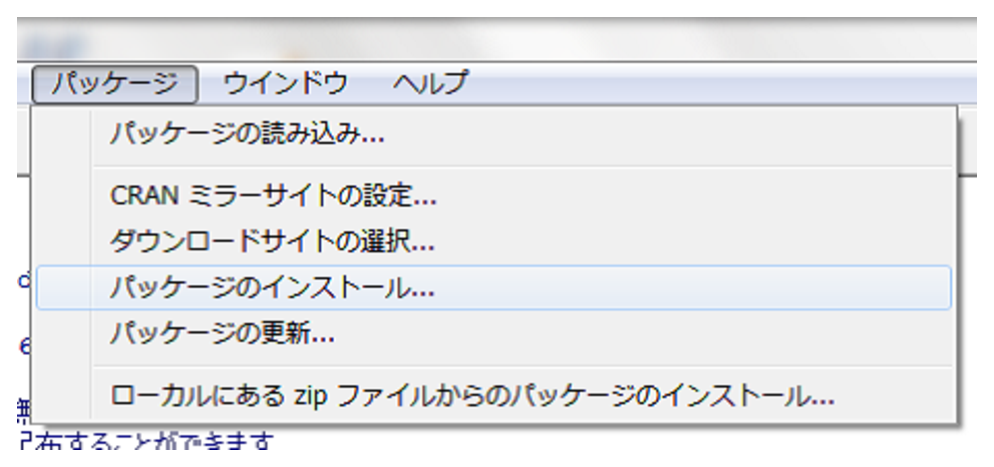
\includegraphics[height=2.5cm]{img/pkg1.eps}\\ \\ \\ \\ \\ \\ \\ \\ \\ \\ \\ \\ \\ \\
        %\end{center}
      \end{minipage}
      % 2
      \begin{minipage}{0.3\hsize}
        %\begin{center}
          CRANのミラーサーバを選択し,\\
          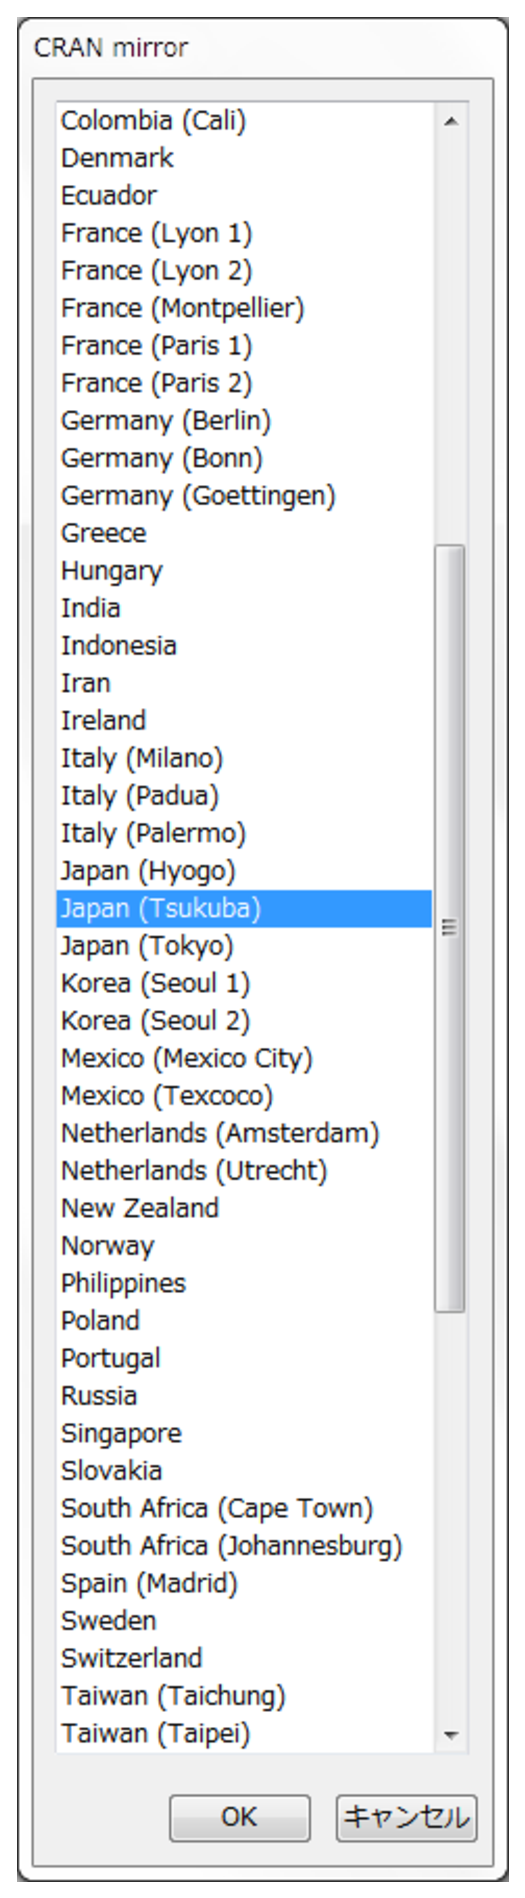
\includegraphics[height=10cm]{img/pkg2.eps}\\

        %\end{center}
      \end{minipage}
      % 3
      \begin{minipage}{0.3\hsize}
        %\begin{center}
          パッケージ一覧から選択するとインストールされる.\\
          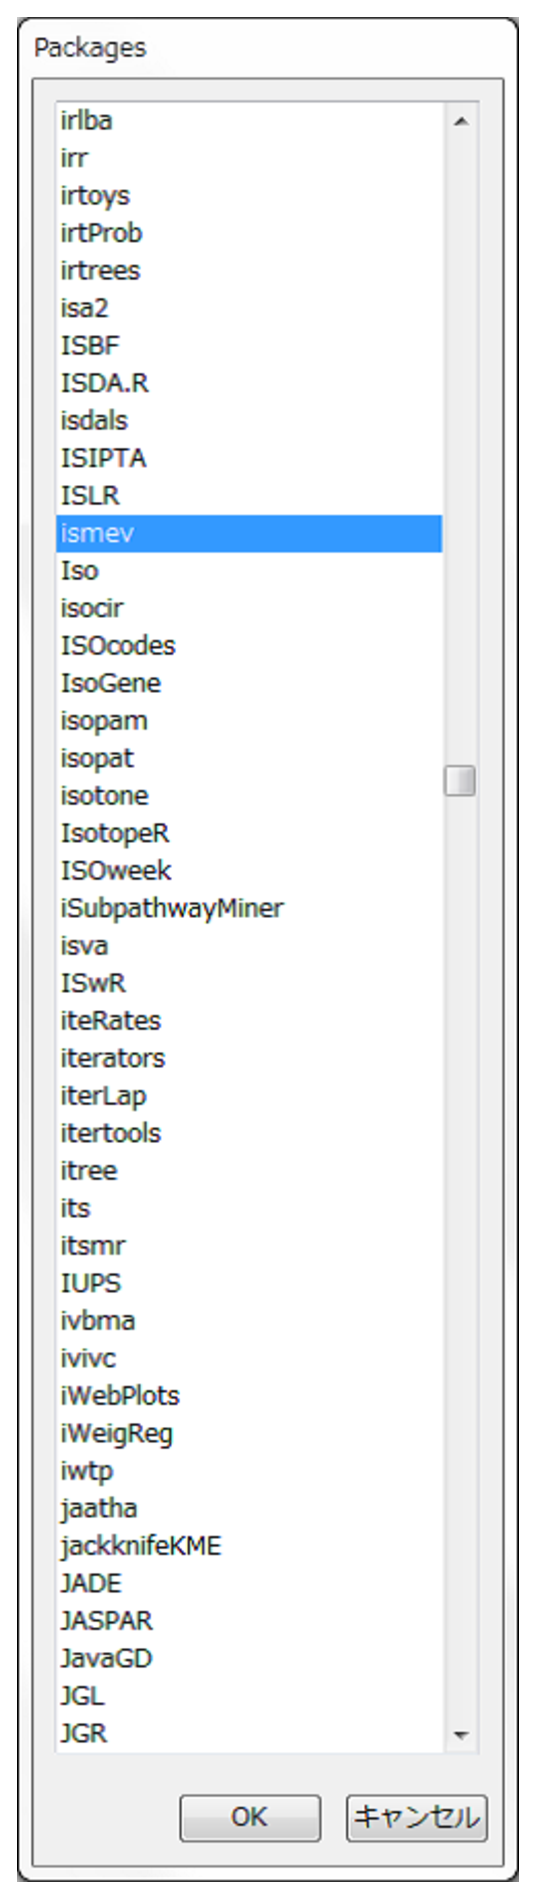
\includegraphics[height=10cm]{img/pkg3.eps}
        %\end{center}
      \end{minipage}
    \end{tabular}
  \end{center}
\end{figure}
\subsection{よくある失敗と対処法}
\subsubsection{プロキシ設定}
研究室のLAN回線ではプロキシサーバーを経由した環境である場合が多い.その場合,Rのパッケージをダウンロードできないため,設定が必要である.
\begin{description}
\item [(Windowsのみ)ショートカットからプロキシの設定の場合]\mbox{}\\
\begin{figure}[H]
  \begin{center}
    \begin{tabular}{c}
      % 1
      \begin{minipage}{0.35\hsize}
        %\begin{center}
          ショートカットを右クリックし,\\プロパティ(R)を開く.\\
          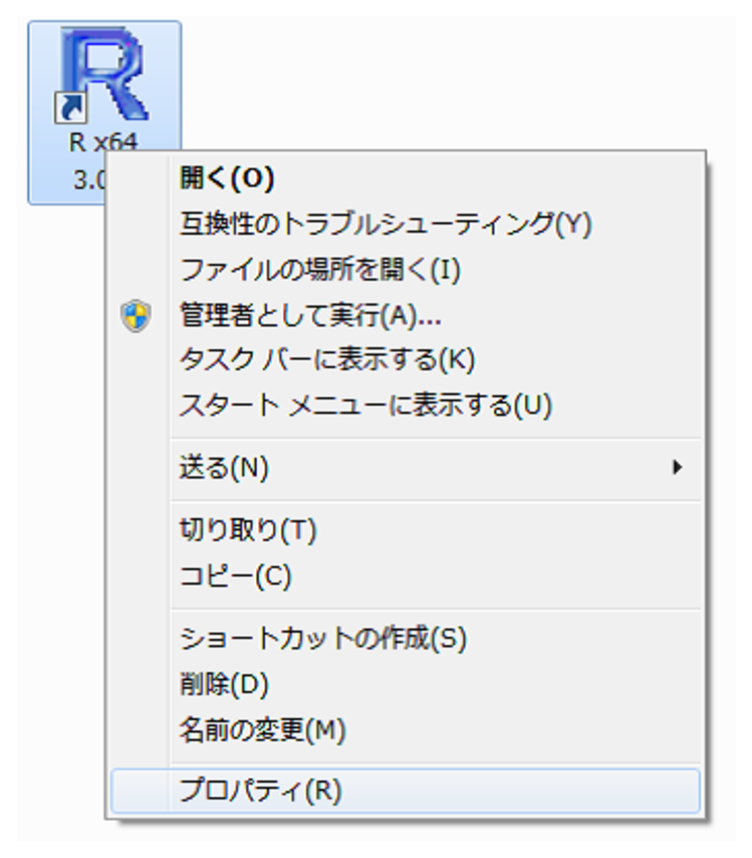
\includegraphics[width=6cm]{img/migi.eps}\\ \\ \\ \\ \\
        %\end{center}
      \end{minipage}
      % 2
      \begin{minipage}{0.65\hsize}
        %\begin{center}
          リンク先(T)のパスの後ろに,\verb+ [スペース]--internet2+を追加し,\\
          \verb+"C:\Program Files\R\R-3.0.1\bin\x64\Rgui.exe --internet2"+\\
          にする.\\
          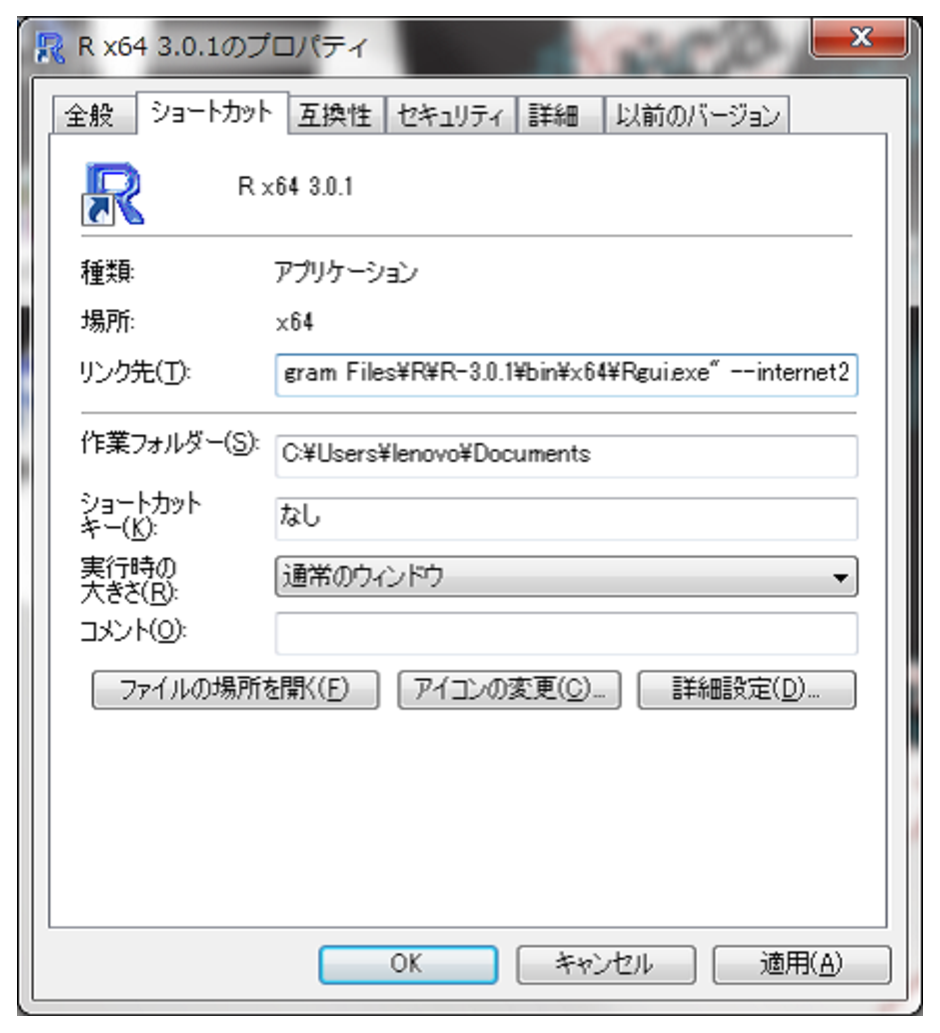
\includegraphics[width=8.2cm]{img/property.eps}
        %\end{center}
      \end{minipage}
    \end{tabular}
  \end{center}
\end{figure}
\item[(すべてのOS)コマンドで設定の場合]\mbox{}\\
\begin{screen}
\begin{verbatim}
Sys.setenv("http_proxy"="http://サーバーアドレス:ポート番号")
\end{verbatim}
\end{screen}
\end{description}
\subsubsection{入力エラー}
また,下の例ように閉じの\verb+"+や\verb+)+を入力せずにEnterを押すと,次の閉じの記号まで,入力待ちになってしまう.この場合,閉じの記号を入力してEnterを押すか,Escを押して先ほどの入力をキャンセルすることができる.
\begin{breakbox}
\begin{verbatim}
> tmp="university
+ 
\end{verbatim}
\end{breakbox}
\newpage
\section{解析してみよう}
\subsection{データの読み込み}
データを格納しているファイル:CSV(カンマ区切りテキスト)やTSV(タブ区切りテキスト)などを読み込む関数がある.
\begin{screen}
\begin{verbatim}
dataA=read.csv(file,header=TRUE,sep=",", skip=0, ...) 
dataB=read.table(file,header=FALSE,sep="",skip=0,...) 
\end{verbatim}
\end{screen}

使用するデータがCSVの場合は{\tt read.csv}関数を使用すればよい.スペース区切りなら{\tt read.table}関数,タブ区切りなら{\tt read.table(file,sep="\verb+\+t")}とする.

また,{\tt header}はテキストにタイトル行がある場合に指定し,{\tt skip}はデータの最初の行にコメント行がある場合読み飛ばす行数を指定する.

{\tt file}の部分はファイルのパスを指定する.面倒な場合は,{\tt file.choose()}とすることでファイルを選択できる.
\begin{screen}
\begin{verbatim}
dataA=read.csv(file.choose()) # ファイル選択ウィンドウが表示される.
\end{verbatim}
\end{screen}
\subsection{回帰分析}
統計的な解析をするうえで,線形回帰分析というものがある.これはデータ$X$とデータ$Y$がどのような関係にあるのかを定量的に式であてはめて分析する手法である.つまり,$Y$を目的変数,$X$を説明変数として,次の式を考える.
\begin{eqnarray*}
Y&=&\alpha +\beta X
\end{eqnarray*}

このように$Y$を$X$で説明するため,最小二乗法という,推定値と観測されたデータの差(残差)の2乗和が最も小さくなる推定を行う.本稿ではデータを生成して,回帰分析を行う.
\begin{breakbox}
\begin{verbatim}
> x2=rnorm(60)
> y2=runif(60,2,4)*x2
> plot(x2,y2)
\end{verbatim}
\begin{center}
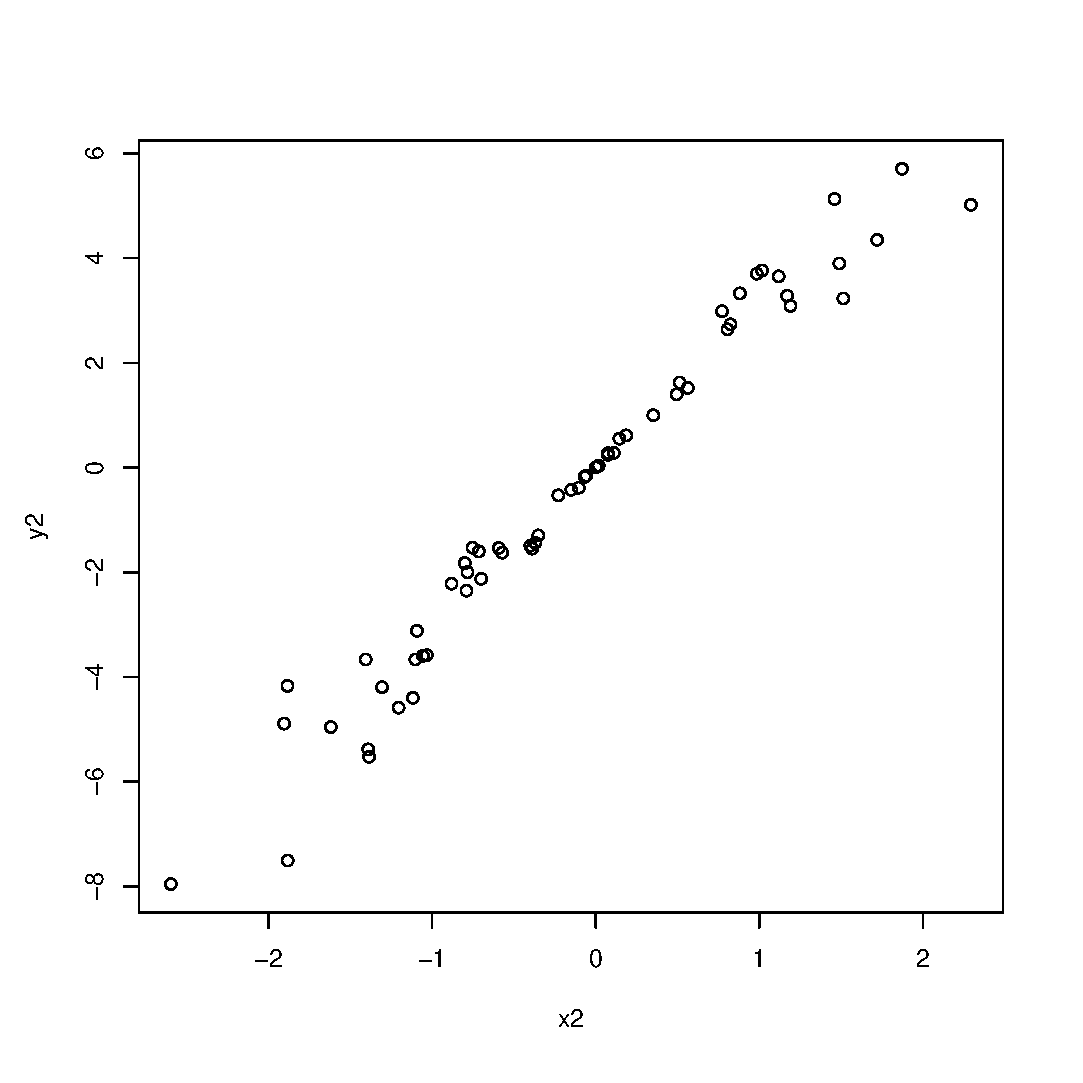
\includegraphics[width=8.2cm]{img/plot2.eps}
\end{center}
\begin{verbatim}
> result2=lm(y2~x2)
> result2

Call:
lm(formula = y2 ~ x2)

Coefficients:
(Intercept)           x2  
   -0.07254      2.98732  
\end{verbatim}
\end{breakbox}
この場合,回帰式は
\begin{eqnarray*}
Y&=&-0.07254-2.98732X
\end{eqnarray*}
となる.この回帰直線を赤線でプロットしたものが以下である.
\begin{breakbox}
\begin{verbatim}
> abline(result2,col=2,lwd=2)
\end{verbatim}
\begin{center}
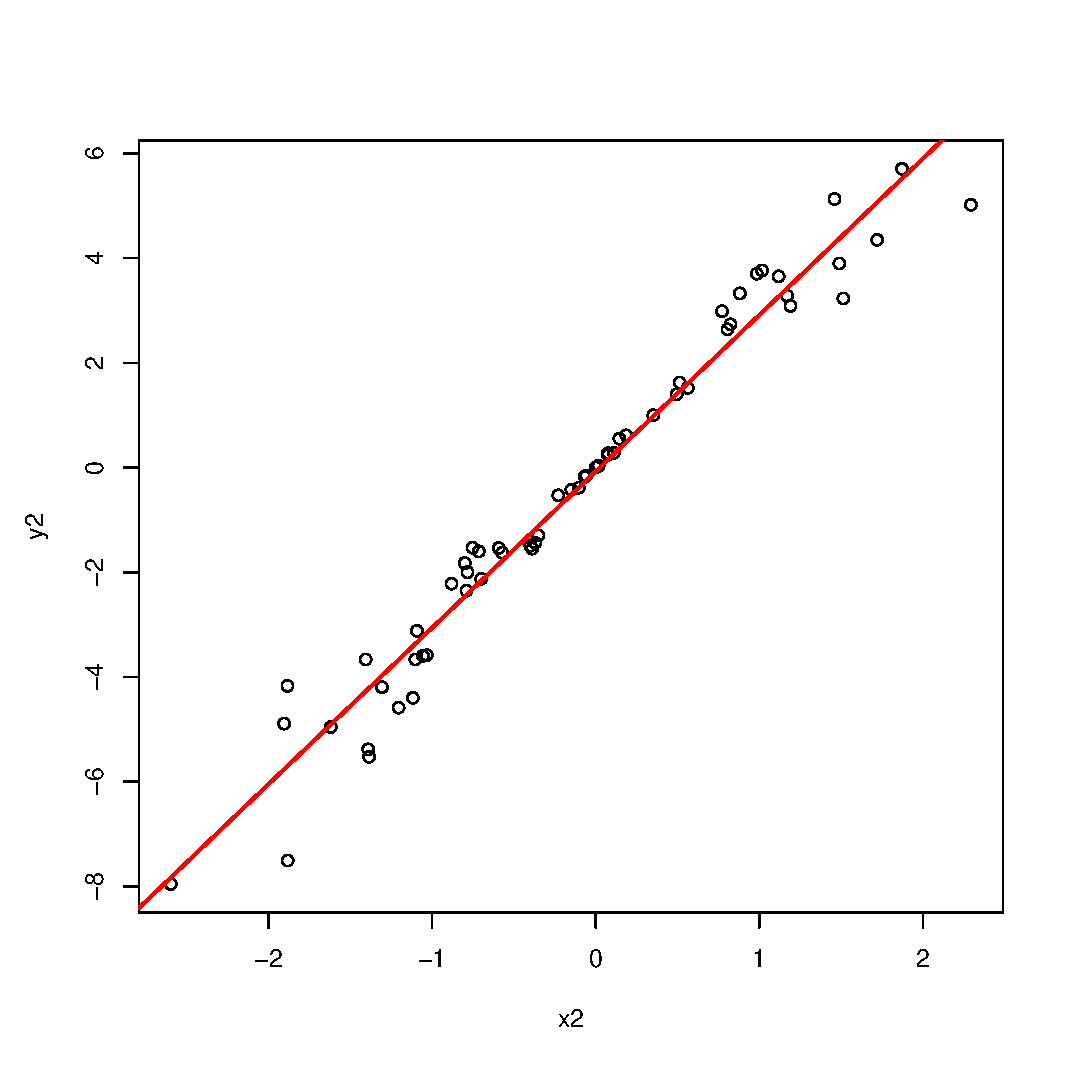
\includegraphics[width=8.2cm]{img/abline2.eps}
\end{center}
\end{breakbox}
また,回帰分析では,係数が$0$と有意に異なるかどうかの検定を行い,係数に意味があるのかを確認する.

{\large 帰無仮説$H_0$:$\beta=0$

対立仮説$H_1$:$\beta \ne 0$}

このような,仮説を立てて帰無仮説が棄却されるかを調べる.
\begin{breakbox}
\begin{verbatim}
> summary(result2)

Call:
lm(formula = y2 ~ x2)

Residuals:
     Min       1Q   Median       3Q      Max 
-1.80981 -0.23454  0.07632  0.31896  1.53236 

Coefficients:
            Estimate Std. Error t value Pr(>|t|)    
(Intercept) -0.07254    0.08324  -0.871    0.387    
x2           2.98732    0.07784  38.380   <2e-16 ***
---
Signif. codes:  0 ‘***’ 0.001 ‘**’ 0.01 ‘*’ 0.05 ‘.’ 0.1 ‘ ’ 1 

Residual standard error: 0.6383 on 58 degrees of freedom
Multiple R-squared: 0.9621,     Adjusted R-squared: 0.9615 
F-statistic:  1473 on 1 and 58 DF,  p-value: < 2.2e-16 
\end{verbatim}
\end{breakbox}
この分散分析表を改めて書きなおしたものが以下である.
\begin{description}
\item[入力された式] \mbox{}\\
\verb+y2 ~ x2+
\item[残差の分布]\mbox{}\\
\begin{tabular}{ccccc}
\noalign{\hrule height 1pt}
最小値&25\%点&中央値&75\%点&最大値\\ \hline
-1.80981&-0.23454&0.07632&0.31896&1.53236 \\
\noalign{\hrule height 1pt}
\end{tabular}
\item[係数]\mbox{}\\
\begin{tabular}{rrrrrl}
\noalign{\hrule height 1pt}
    &\multicolumn{1}{c}{推定値}&\multicolumn{1}{c}{標準誤差}&\multicolumn{1}{c}{t値}&\multicolumn{1}{c}{P-値($Pr( t_0>|t|)$)}& \\ \hline
切片&-0.07254& 0.08324&-0.871&0.387& \\
  x1&2.98732&  0.07784& 38.380 &$<2\times 10^{-16}$ &*** \\
\noalign{\hrule height 1pt}
\end{tabular}

*** は有意水準0.001で有意であるということ.\\
有意水準0.001で帰無仮説$H_0$:$\beta=0$が棄却された.P-値が$<2\times 10^{-16}$とは帰無仮説が正しいときに,帰無仮説を棄却する確率が$2\times 10^{-16}$以下ということである.
\item[回帰統計]\mbox{}\\
\begin{tabular}{lr}
\noalign{\hrule height 1pt}
標準誤差&0.6282(自由度58)\\
決定係数$R^2$&0.9621\\
自由度調整済決定係数$R^2$&0.9615\\
F値(観測された分散比)&1473(自由度1と58)\\
P-値&$<2\times 10^{-16}$\\
\noalign{\hrule height 1pt}
\end{tabular}

ここのP-値ではすべての係数が0であるという帰無仮説の検定となっている.
\end{description}

次に,バラバラなデータを解析する.
\begin{breakbox}
\begin{verbatim}
> x1=rnorm(60)
> y1=rnorm(60)
> plot(x1,y1)
\end{verbatim}
\begin{center}
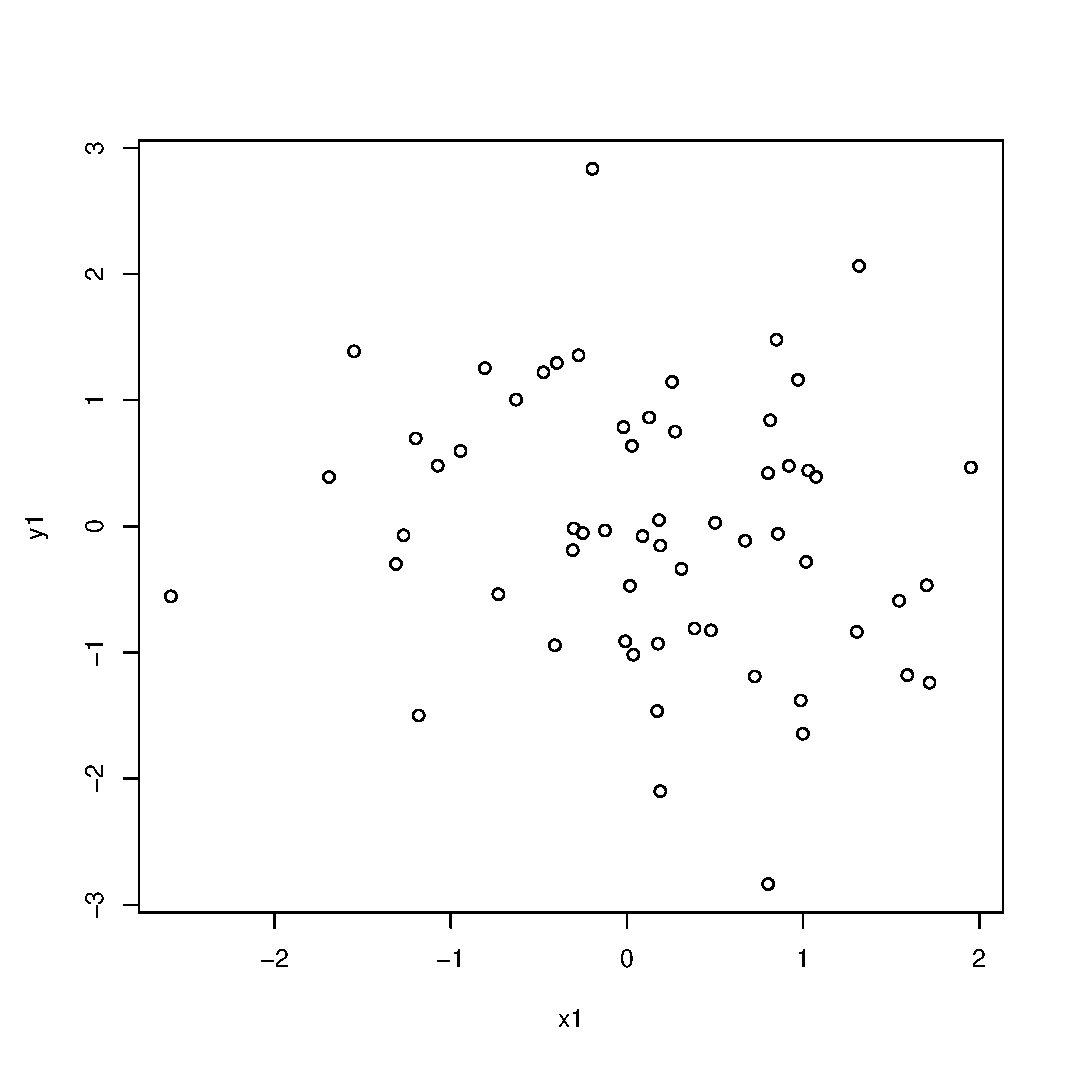
\includegraphics[width=8.2cm]{img/plot1.eps}
\end{center}
\end{breakbox}
このように先ほどと違い,点がバラバラである.
\begin{breakbox}
\begin{verbatim}
> result1=lm(y1~x1)
> result1

Call:
lm(formula = y1 ~ x1)

Coefficients:
(Intercept)           x1  
    0.01997     -0.18988  
\end{verbatim}
\end{breakbox}
この場合,回帰式は
\begin{eqnarray*}
Y&=&0.01997-0.18988X
\end{eqnarray*}
である.この回帰式を赤線でプロットしたものが下図である.
\begin{center}
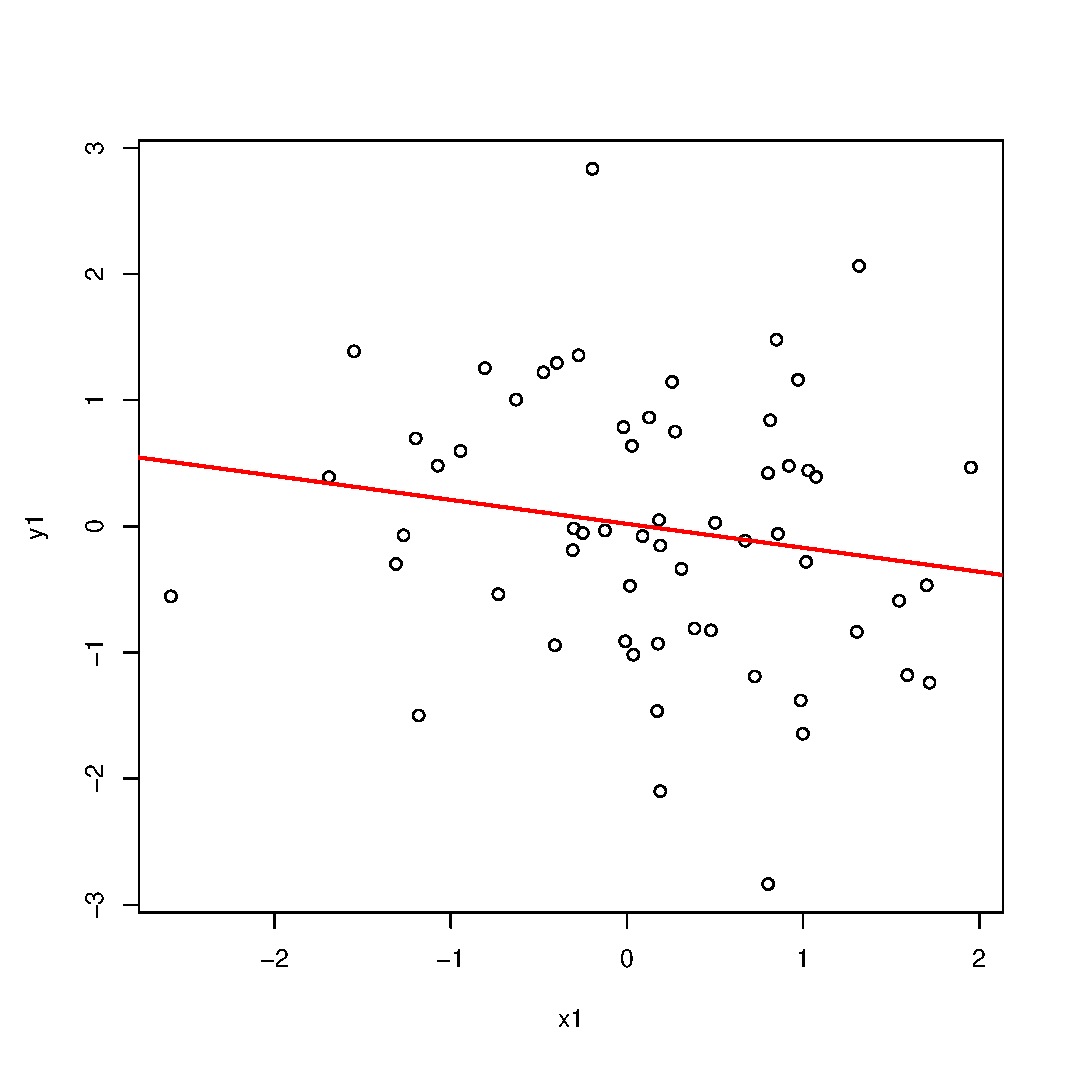
\includegraphics[width=8.2cm]{img/abline1.eps}
\end{center}

あまり意味のない線のように見える.そこで,先ほどと同様に分散分析表を確認する.
\begin{breakbox}
\begin{verbatim}
> summary(result1)

Call:
lm(formula = y1 ~ x1)

Residuals:
     Min       1Q   Median       3Q      Max 
-2.70223 -0.75451 -0.07851  0.76754  2.77611 

Coefficients:
            Estimate Std. Error t value Pr(>|t|)
(Intercept)  0.01997    0.13663   0.146    0.884
x1          -0.18988    0.14523  -1.307    0.196

Residual standard error: 1.044 on 58 degrees of freedom
Multiple R-squared: 0.02863,    Adjusted R-squared: 0.01188 
F-statistic: 1.709 on 1 and 58 DF,  p-value: 0.1962 
\end{verbatim}
\end{breakbox}
つまりこの結果は以下であり,
\begin{description}
\item[入力された式] \mbox{}\\
\verb+y1 ~ x1+
\item[残差の分布]\mbox{}\\
\begin{tabular}{ccccc}
\noalign{\hrule height 1pt}
最小値&25\%点&中央値&75\%点&最大値\\ \hline
-2.70223&-0.75451&-0.07851&0.76754& 2.77611 \\
\noalign{\hrule height 1pt}
\end{tabular}
\item[係数]\mbox{}\\
\begin{tabular}{rrrrr}
\noalign{\hrule height 1pt}
    &\multicolumn{1}{c}{推定値}&\multicolumn{1}{c}{標準誤差}&\multicolumn{1}{c}{t値}&\multicolumn{1}{c}{P-値($Pr( t_0>|t|)$)} \\ \hline
切片& 0.01997& 0.13663& 0.146&0.884 \\
  x1&-0.18988& 0.14523&-1.307&0.196 \\
\noalign{\hrule height 1pt}
\end{tabular}

帰無仮説が棄却されていないのがわかる.
\item[回帰統計]\mbox{}\\
\begin{tabular}{lr}
\noalign{\hrule height 1pt}
標準誤差&1.044(自由度58)\\
決定係数$R^2$&0.02863\\
自由度調整済決定係数$R^2$&0.01188\\
F値(観測された分散比)&1.709(自由度1と58)\\
P-値&0.1962\\
\noalign{\hrule height 1pt}
\end{tabular}

ここのP-値も大きい.
\end{description}
\subsubsection{{\tt lm}関数について}
{\tt lm}関数は以下のように使用する.
\begin{screen}
\begin{verbatim}
lm(formula , data,...)
\end{verbatim}
\end{screen}
\begin{description}
\item[{\tt formula}の指定方法] \mbox{} 
\begin{center}
\begin{tabular}{l|p{11.6cm}}
\noalign{\hrule height 1pt}
 \multicolumn{1}{c|}{{\tt formula}} & \multicolumn{1}{c}{回帰モデル式}\\ \hline
 \verb|y~x| &$y=\alpha +\beta x+\epsilon$ \\ 
 \verb|y~x1+x2| &$y=\alpha +\beta_1 x_1+\beta_2 x_2 +\epsilon$ \\ 
 \verb|y~x1*x2| & $y=\alpha +\beta_1 x_1+\beta_2 x_2+\beta_3 x_1 x_2+ +\epsilon$\\ 
 \verb|y~x1+x2+x1*x2| & \hspace{6em}〃\\ 
 \verb|y~(x1+x2)^2| & \hspace{6em}〃\\ 
 \verb|y~x-1| & $y=\beta x +\epsilon$ (定数項なし)\\ 
 \verb|y~x+0| & \hspace{6em}〃\\ 
 \verb|y~x+I(x^2)| & $y=\alpha+\beta_1 x+\beta_2 x^2+\epsilon$\\ 
 \verb|y~. , data=データ名| &指定したデータに含まれる{\tt y}を目的変数,{\tt y}以外の変数すべてを説明変数に指定する.($y=\alpha+\beta_1 x_1+\cdots+\beta_p x_p +\epsilon$) \\ 
\noalign{\hrule height 1pt}
\end{tabular}
\end{center}

なお,$\epsilon$は誤差項のことである.
\end{description}

lm関数が返すオブジェクトには,以下の情報が含まれるが特に覚える必要はない.
\begin{breakbox}
\begin{verbatim}
> result=lm(y2~x2)
> str(result)
List of 12
 $ coefficients : Named num [1:2] -0.0725 2.9873
  ..- attr(*, "names")= chr [1:2] "(Intercept)" "x2"
 $ residuals    : Named num [1:60] 0.6062 0.6405 -0.0037 0.7905 0.131 ...
  ..- attr(*, "names")= chr [1:60] "1" "2" "3" "4" ...
 $ effects      : Named num [1:60] 4.0488 24.4985 -0.0605 0.6912 0.0932 ...
  ..- attr(*, "names")= chr [1:60] "(Intercept)" "x2" "" "" ...
 $ rank         : int 2
 $ fitted.values: Named num [1:60] -4.272 -2.465 -0.381 -2.321 0.484 ...
  ..- attr(*, "names")= chr [1:60] "1" "2" "3" "4" ...
 $ assign       : int [1:2] 0 1
 $ qr           :List of 5
  ..$ qr   : num [1:60, 1:2] -7.746 0.129 0.129 0.129 0.129 ...
  .. ..- attr(*, "dimnames")=List of 2
  .. .. ..$ : chr [1:60] "1" "2" "3" "4" ...
  .. .. ..$ : chr [1:2] "(Intercept)" "x2"
  .. ..- attr(*, "assign")= int [1:2] 0 1
  ..$ qraux: num [1:2] 1.13 1.06
  ..$ pivot: int [1:2] 1 2
  ..$ tol  : num 1e-07
  ..$ rank : int 2
  ..- attr(*, "class")= chr "qr"
 $ df.residual  : int 58
 $ xlevels      : Named list()
 $ call         : language lm(formula = y2 ~ x2)
 $ terms        :Classes 'terms', 'formula' length 3 y2 ~ x2
  .. ..- attr(*, "variables")= language list(y2, x2)
  .. ..- attr(*, "factors")= int [1:2, 1] 0 1
  .. .. ..- attr(*, "dimnames")=List of 2
  .. .. .. ..$ : chr [1:2] "y2" "x2"
  .. .. .. ..$ : chr "x2"
  .. ..- attr(*, "term.labels")= chr "x2"
  .. ..- attr(*, "order")= int 1
  .. ..- attr(*, "intercept")= int 1
  .. ..- attr(*, "response")= int 1
  .. ..- attr(*, ".Environment")=<environment: R_GlobalEnv> 
  .. ..- attr(*, "predvars")= language list(y2, x2)
  .. ..- attr(*, "dataClasses")= Named chr [1:2] "numeric" "numeric"
  .. .. ..- attr(*, "names")= chr [1:2] "y2" "x2"
 $ model        :'data.frame':	60 obs. of  2 variables:
  ..$ y2: num [1:60] -3.666 -1.825 -0.385 -1.531 0.615 ...
  ..$ x2: num [1:60] -1.406 -0.801 -0.103 -0.753 0.186 ...
  ..- attr(*, "terms")=Classes 'terms', 'formula' length 3 y2 ~ x2
  .. .. ..- attr(*, "variables")= language list(y2, x2)
  .. .. ..- attr(*, "factors")= int [1:2, 1] 0 1
  .. .. .. ..- attr(*, "dimnames")=List of 2
  .. .. .. .. ..$ : chr [1:2] "y2" "x2"
  .. .. .. .. ..$ : chr "x2"
  .. .. ..- attr(*, "term.labels")= chr "x2"
  .. .. ..- attr(*, "order")= int 1
  .. .. ..- attr(*, "intercept")= int 1
  .. .. ..- attr(*, "response")= int 1
  .. .. ..- attr(*, ".Environment")=<environment: R_GlobalEnv> 
  .. .. ..- attr(*, "predvars")= language list(y2, x2)
  .. .. ..- attr(*, "dataClasses")= Named chr [1:2] "numeric" "numeric"
  .. .. .. ..- attr(*, "names")= chr [1:2] "y2" "x2"
 - attr(*, "class")= chr "lm"
\end{verbatim}
\end{breakbox}
\begin{description}
\item[返り値に含まれる主なオブジェクトとそれを利用する関数]\mbox{}\\
ここでは,\verb+result=lm(y2~x2)+とした場合の{\tt result}のことである.
\begin{itemize}
\item モデル式 \\
先ほど説明した {\tt formula}を指す.\verb+result$call+で取り出すことができる.
\item 係数 \\
\verb+result$coefまたは+\verb+result$coefficient+や\verb+coef(result)+で取り出すことができる.
\item 残差\\
観測値と推定したモデルとの誤差.\verb+result$residual+や\verb+result$residuals+や\verb+result$resid+や\\
\verb+residuals(result)+や\verb+resid(result)+で取り出すことができる.
\item 残差平方和\\
数式で表すと$\sum \limits ^n _{i=1} \left( y-\hat{y} \right)$.\verb+deviance(result)+で取り出すことができる.また,\verb+sum(result2$resid^2)+とするのと同じである.
\item 推定値\\
\verb+predict(result)+でモデルに当てはめた値,つまり$y_2$の推定値$\hat{y_2}$を得る.また,\verb+predict(result,newdata=データ名)+とすることで予測を行うこともできる.つまり,$\mbox{残差}=\mbox{観測値}-\mbox{推定値}$ということである.\\
※ データには回帰分析を行ったデータと同じ変数が存在する必要がある.
\item 作図\\
\verb+plot(result)+とすると4つ作図される.以下にそれぞれの説明を記す.
\end{itemize}
\begin{indentation}{3em}{0pt}
\begin{enumerate}
\item 残差と推定値の散布図\\
図の横軸が推測値,縦軸が残差である.この図から残差の全体像を確認することができる.
\begin{center}
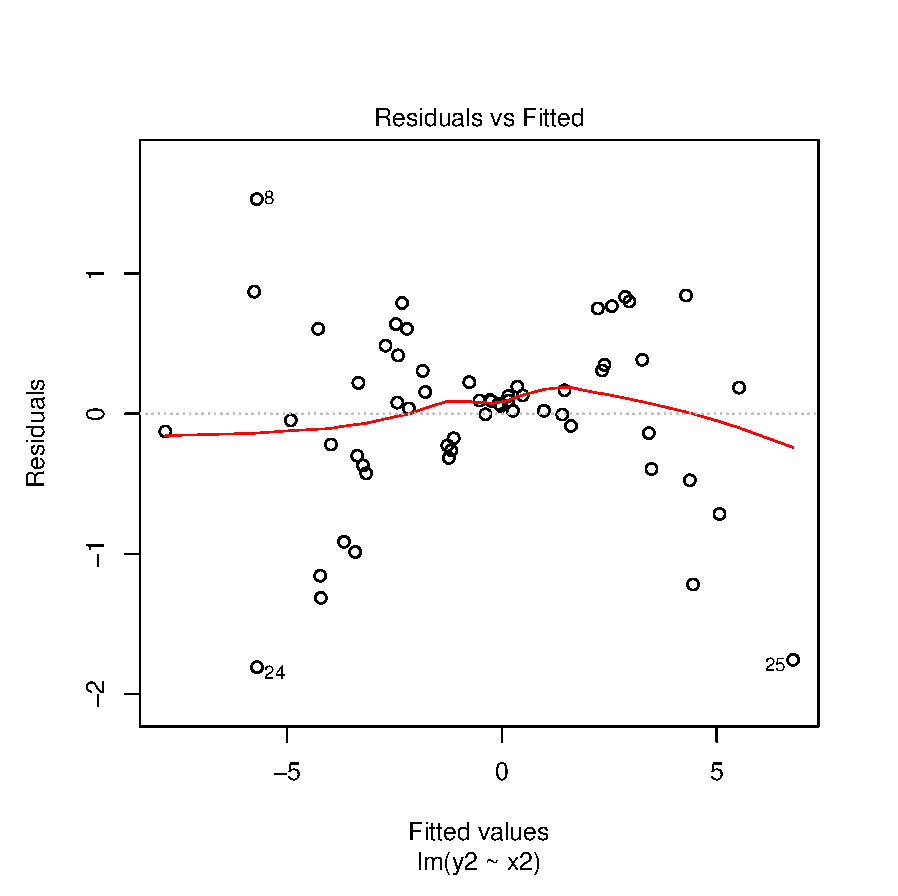
\includegraphics[width=11cm]{img/plotlm1.eps}
\end{center}
\item 残差の正規QQプロット\\
正規QQプロットじゃデータの正規性を考察するためにデータを視覚化する方法.データが正規分布に従う場合,点が一直線上に並べられる.
\begin{center}
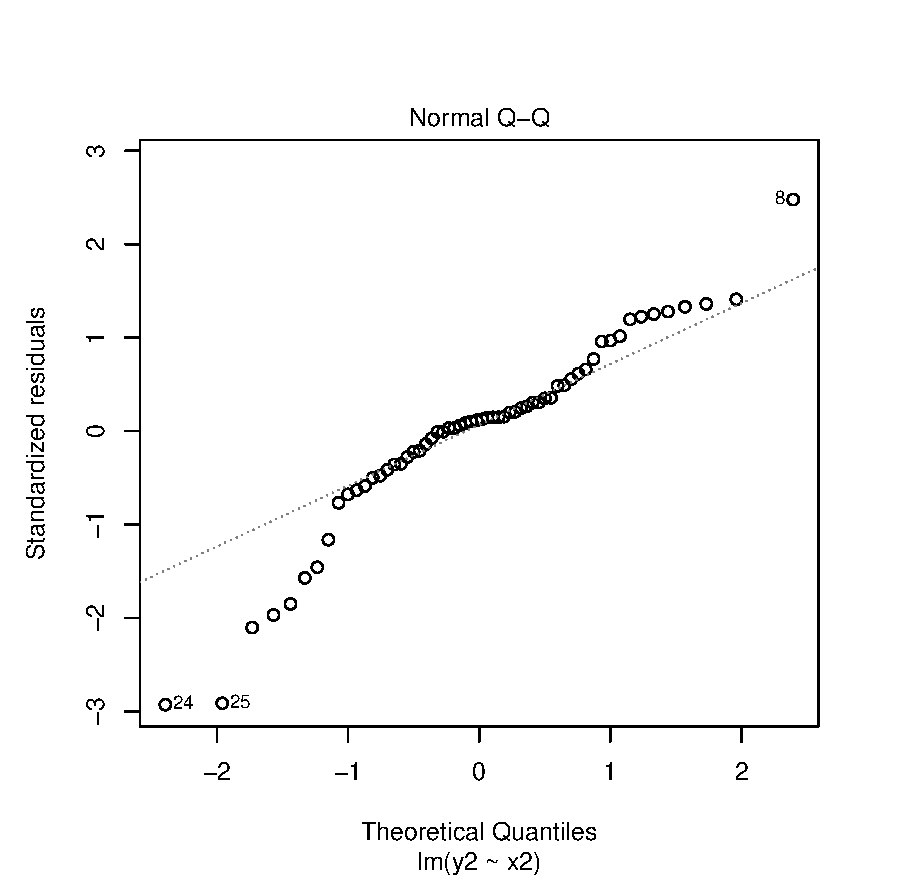
\includegraphics[width=11cm]{img/plotlm2.eps}
\end{center}
\item Scale-Location図\\
標準化した残差の絶対値の平方根を縦軸にし,推測値を横軸とした散布図.
\begin{center}
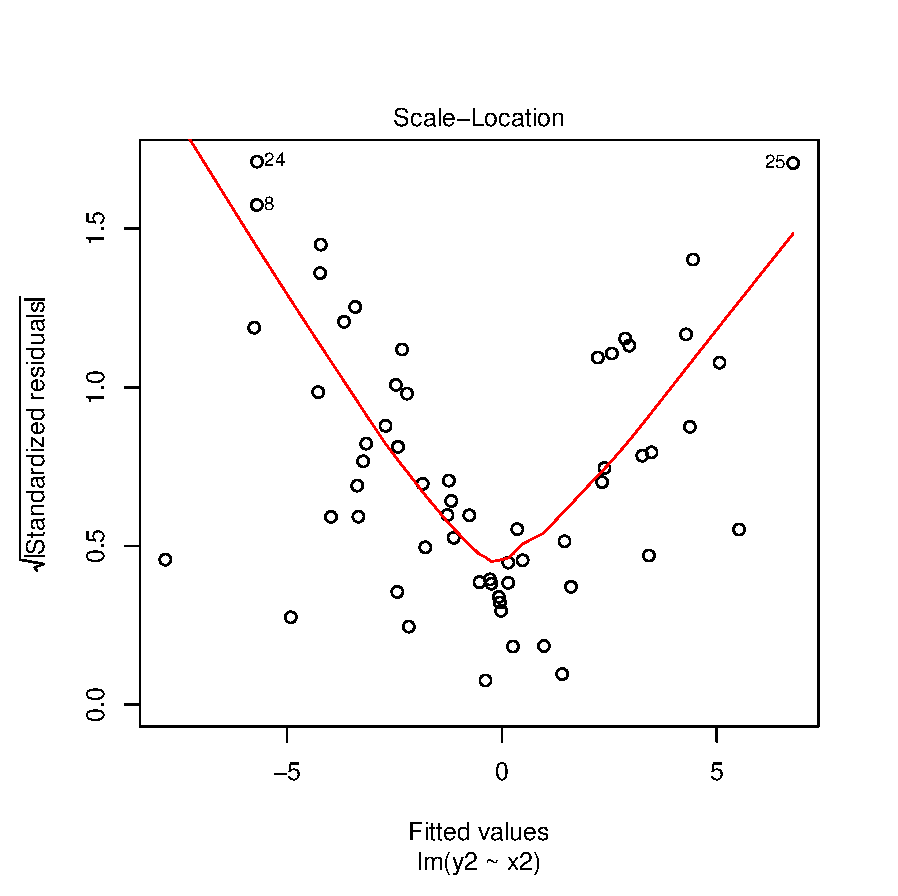
\includegraphics[width=11cm]{img/plotlm3.eps}
\end{center}
\item 残差-てこ比\\
てこ比は観測値が推測値に及ぼす影響の大きさである.クックの距離は,各データがどれだけ推定に影響を与えているかを示す指標.
\begin{center}
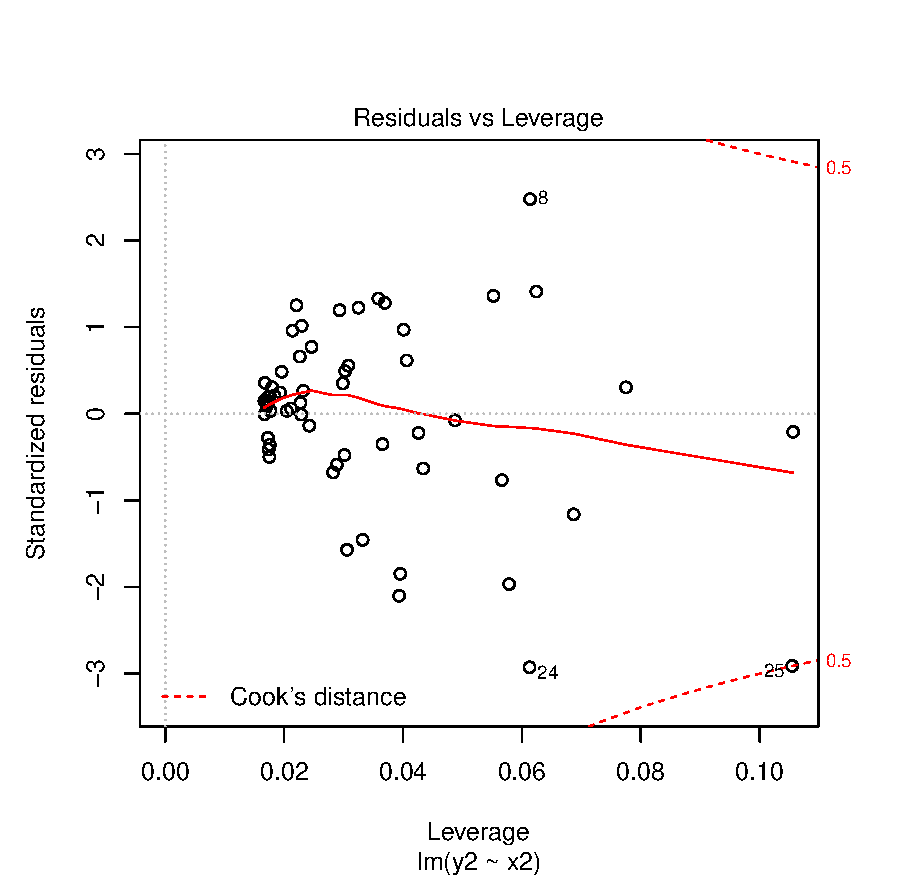
\includegraphics[width=11cm]{img/plotlm4.eps}
\end{center}
\end{enumerate}
\end{indentation}
\end{description}
\subsubsection{補遺}
\begin{description}
\item[平均]\mbox{}\\
\begin{eqnarray*}
\bar{x}&=&\frac{1}{n}\sum \limits ^n_{i=1}x_i
\end{eqnarray*}
\item[分散]\mbox{}\\
\begin{eqnarray*}
s^2 &=& \frac{1}{n} \sum_{i=1}^{n}(x_i - \bar{x})^2 \\
    &=& \bar{x^2}-\left( \bar{x} \right)^2
\end{eqnarray*}
これを{\bf 標本分散}という.
\item[不偏分散]\mbox{}\\
上記の分散は,$\displaystyle E[s^2] = \frac{n-1}{n} \sigma^2 (\sigma^2\mbox{は母集団の分散})$とした場合,標本の分散は母集団の分散よりも小さくなる傾向がある.すなわち,標本の分散は母集団の分散の不偏推定量ではない.不偏分散は以下の式で表される.また,Rの{\tt var}関数では不偏分散が採用されている.標本数が十分に大きければ標本分散とほぼ等しくなる.
\begin{eqnarray*}
u^2 &=& \frac{1}{n-1} \sum_{i=1}^{n}(x_i - \bar{x})^2 
\end{eqnarray*}
\item[標準偏差]\mbox{}\\
\begin{eqnarray*}
\sqrt{\mathrm{V}(X)}
\end{eqnarray*}
つまり,分散の正の平方根.
\item[共分散]\mbox{}\\
\begin{eqnarray*}
\mathrm{Cov}(X, Y)&=&\frac{1}{n}\sum_{i=1}^{n} (x_{i}-\bar{x})(y_{i}-\bar{y})\\
&=& \frac{S_{xy}}{n}
\end{eqnarray*}
\item[相関係数]\mbox{}\\
\begin{eqnarray*}
\mathrm{Cor}(X,Y)&=&\frac{\mathrm{Cov}(X,Y)}{\sqrt{\mathrm{V}(X)}\sqrt{\mathrm{V}(Y)}}\\
&=&\frac{ \displaystyle \sum_{i=1}^{n} (x_{i}-\bar{x})(y_{i}-\bar{y}) }{ \displaystyle \sqrt{\sum_{i=1}^n(x_{i}-\bar{x})^2} \sqrt{\sum_{i=1}^n(y_{i}-\bar{y})^2}}
\end{eqnarray*}
つまり,共分散をそれぞれの標準偏差で割ったもの.
\item[最小二乗法]\mbox{}\\
$y_i$の推定値を$\hat{y_i}=\alpha+\beta x_i$とした場合,実際の観測値と推定値の差を残差と呼ぶ.残差を$e_i$
で表すと,
\begin{eqnarray*}
e_i&=&y_i-\hat{y}\\
&=&y_i-\left( \alpha+\beta x_i \right)
\end{eqnarray*}
であり,最小二乗法は残差平方和を最小にする方法である.残差平方和を$\alpha$と$\beta$の関数とみなすと以下のように表せる.
\begin{eqnarray*}
S_e(\alpha,\beta)&=&\sum \limits ^n _{i=1}e_i ^2\\
&=&\sum \limits ^n _{i=1}\left( y_i-\alpha-\beta x_i \right)
\end{eqnarray*}
$S(\alpha,\beta)$は$\alpha,\beta$に関する2次関数で,$S(\alpha,\beta)$を最小化する$\alpha,\beta$を見つけるには微分すれば良い.

まず,$\alpha$に関して微分する.
\begin{eqnarray*}
\frac{\partial S}{\partial \alpha}&=&-2\sum\limits ^n_{i=1}\left( y_i-\alpha-\beta x_i \right)=0
\end{eqnarray*}
これを変形する.
\begin{eqnarray*}
\sum\limits ^n_{i=1}y_i&=&\sum\limits ^n_{i=1}\alpha+\sum\limits ^n_{i=1}\beta x_i
\end{eqnarray*}
両辺を$n$で割る.
\begin{eqnarray}
\bar{y}&=&\alpha+\beta\bar{x} \label{alpha}
\end{eqnarray}
また,$\beta$に関して微分する.
\begin{eqnarray*}
\frac{\partial S}{\partial \beta}&=&-2\sum\limits ^n_{i=1}\left( y_i-\alpha-\beta x_i \right)x_i=0
\end{eqnarray*}
変形し,
\begin{eqnarray}
\sum\limits ^n_{i=1}x_i y_i&=&\alpha \sum\limits ^n_{i=1}x_i+\beta\sum\limits ^n_{i=1}\beta x_i^2 \label{beta}
\end{eqnarray}
(\ref{alpha})(\ref{beta})の連立方程式より$\alpha$と$\beta$について解く.(\ref{alpha})を$\alpha$について解き,(\ref{beta})に代入する.
\begin{eqnarray*}
\sum \limits ^n_{i=1}x_i y_i&=&\left( \bar{y}-\beta \bar{x} \right)\sum \limits ^n_{i=1}x_i +b\sum \limits ^n_{i=1}x_i^2 \\
&=&n\bar{x}\bar{y}+b\left( \sum \limits ^n_{i=1}x_i^2 - n\bar{x}^2 \right)
\end{eqnarray*}
また,以下の式が得られる.
\begin{eqnarray*}
S_{xy}&=&\beta S_{xx}
\end{eqnarray*}
ただし,$S_{xx}$と$S_{xy}$は以下である.
\begin{eqnarray*}
S_{xx}&=&\sum \limits^n _{i=1}\left( x_i -\bar{x} \right)^2=\sum \limits^n _{i=1}x_i^2-n\bar{x}\\
S_{xy}&=&\sum \limits^n _{i=1}\left( x_i-\bar{x} \right)\left( y_i - \bar{y} \right)=\sum \limits^n _{i=1}x_i y_i -n\bar{x}\bar{y}
\end{eqnarray*}
以上より,(\ref{estalpha})と(\ref{estbeta})を得る.
\begin{eqnarray}
\alpha&=&\bar{y}-b\bar{x} \label{estalpha}\\
\beta  &=&\frac{S_{xy}}{S_{xx}} \label{estbeta}
\end{eqnarray}
また,細かな計算は省略するが行列計算を行うことで,最小二乗法によって係数を求めることもできる.
$Y$を目的変数の$n$行1列の行列としてとして,$X$を説明変数の$n$行2列\footnote[1]{この行列$X$の左に成分がすべて1の行を結合して定数項を推定している.}として,$Y=X\beta$となる行列$\beta$を求める.
\begin{eqnarray*}
\beta=(X^T X)^{-1}X^T Y
\end{eqnarray*}
Rでは\verb+beta=solve(t(x)%*%x)%*%t(x)%*%y+と表現する.
\item[決定係数]\mbox{}\\
残差平方和を$S_e=\sum \limits^n _{i=1} e_i^2$とする.目的変数$y$の偏差平方和を$S_{yy}=\sum \limits^n _{i=1}\left( y_i -\bar{y} \right)^2=\sum \limits^n _{i=1}y_i^2-n\bar{y}$とする.
\begin{eqnarray*}
R^2&=&1-\frac{S_E}{S_{yy}}
\end{eqnarray*}
また,寄与率とも言う.説明変数が目的変数をどの程度説明できるかを表す.標本値から求めた回帰方程式のあてはまりの良さの尺度である.
\item[自由度調整済み決定係数]\mbox{}\\
説明変数を増やすと決定係数は大きくなるため,サンプル数を$n$,データの中の説明変数の数を$k$として,自由度を調整した決定係数が以下である.
\begin{eqnarray*}
(adjusted\ R^2)&=&1-\frac{S_E /(n-k-1)}{S_{yy} /(n-1)}
\end{eqnarray*}
\item[標準誤差]\mbox{}\\
残差の不偏分散を以下とする.
\begin{eqnarray*}
S_e^2&=&\frac{S_e}{n-k-1}
\end{eqnarray*}
係数$\alpha$,$\beta$の標準誤差SE$(\alpha)$,$SE(\beta)$は以下で求められる.
\begin{eqnarray*}
SE(\alpha)&=&\sqrt{S_e^2 \left[\frac{1}{n}+\frac{\bar{x}^2}{\sum \limits ^n _{i=1}\left( x_i-\bar{x} \right)}\right]}\\
SE(\beta)&=&\sqrt{\frac{S_e^2}{\sum \limits ^n _{i=1}\left( x_i-\bar{x} \right)}}
\end{eqnarray*}
\item[t値]\mbox{}\\
係数$\alpha$,$\beta$のt値は以下である.
\begin{eqnarray*}
t_\alpha &=&\frac{\alpha}{SE(\alpha)}\\
t_\beta &=&\frac{\beta}{SE(\beta)}
\end{eqnarray*}
このt値に対応するp値は{\tt pt}関数で求めることができる.t値は帰無仮説:係数が0であるという仮説検定の統計量である.p値が有意水準(0.05,0.01,0.005)よりも小さい場合は,p値の右側にそれぞれ(*,**,***)を付ける.
\item[F値]\mbox{}\\
F値は帰無仮説:すべての係数が0であるという仮説検定の統計量である.F値は決定係数から求められ,自由度$k$,$n-k-1$のF分布に従う.
\begin{eqnarray*}
F&=&\frac{R^2}{1-R^2}\times\frac{n-k-1}{k}
\end{eqnarray*}
\end{description}\end{document}
\section{演習問題}
\begin{enumerate}
\item 平均2,分散2の正規乱数を10000個生成して,その平均と分散を計算せよ.
\item 平均0,分散4の正規乱数を10個生成し,平均を推定する.この操作を10000回繰り返し,10000個の平均値の平均と分散を計算せよ.このとき,10000個の平均値 の分散は理論上どんな値となると考えられるか考察せよ.
\item Rにインストールされているデータフレーム{\tt faithful}について,横軸に{\tt waiting},縦軸に{\tt eruptions}をとった散布図を描け.散布の名前は「待ち時間と噴出継続時間の関係」とせよ.
\item データフレーム{\tt faithful}において,待ち時間で噴出継続時間との関係を表す回帰直線を求め,散布図に赤色の直線を上書きせよ.\label{mon4}
\item 問\ref{mon4}で4.5分以上の間欠泉を見るには何分以上待つことが妥当か考察せよ.
\item 3つの自然数$m<n<k\leq100$に対して,$m^2 +n^2 =k^2$を満足する組み合わせをすべて求めよ.また,$m, n, k$ を三角形の一辺とする直角三角形を考えたとき,相似図形を一種類と考えて何種類の三角形が作れるか.すべての組み合わせを求めよ.
\end{enumerate}
